% Adicione no preâmbulo do documento principal: \usepackage{amssymb}

\chapter{RESULTADOS E DISCUSSÃO}

Este capítulo apresenta os resultados obtidos com a implementação do sistema Investe-AI, incluindo as métricas de desempenho das duas redes neurais artificiais desenvolvidas: a primeira para classificação de perfil de risco e a segunda para recomendação de alocação de carteiras de investimento.

\section{Sistema Dual de Redes Neurais}

O sistema implementado utiliza uma arquitetura dual, onde duas redes neurais trabalham de forma integrada e sequencial para fornecer recomendações personalizadas de investimento. A Figura~\ref{fig:arquitetura_rede} ilustra a arquitetura completa do sistema com as duas redes neurais.

\begin{figure}[htbp]
    \centering
    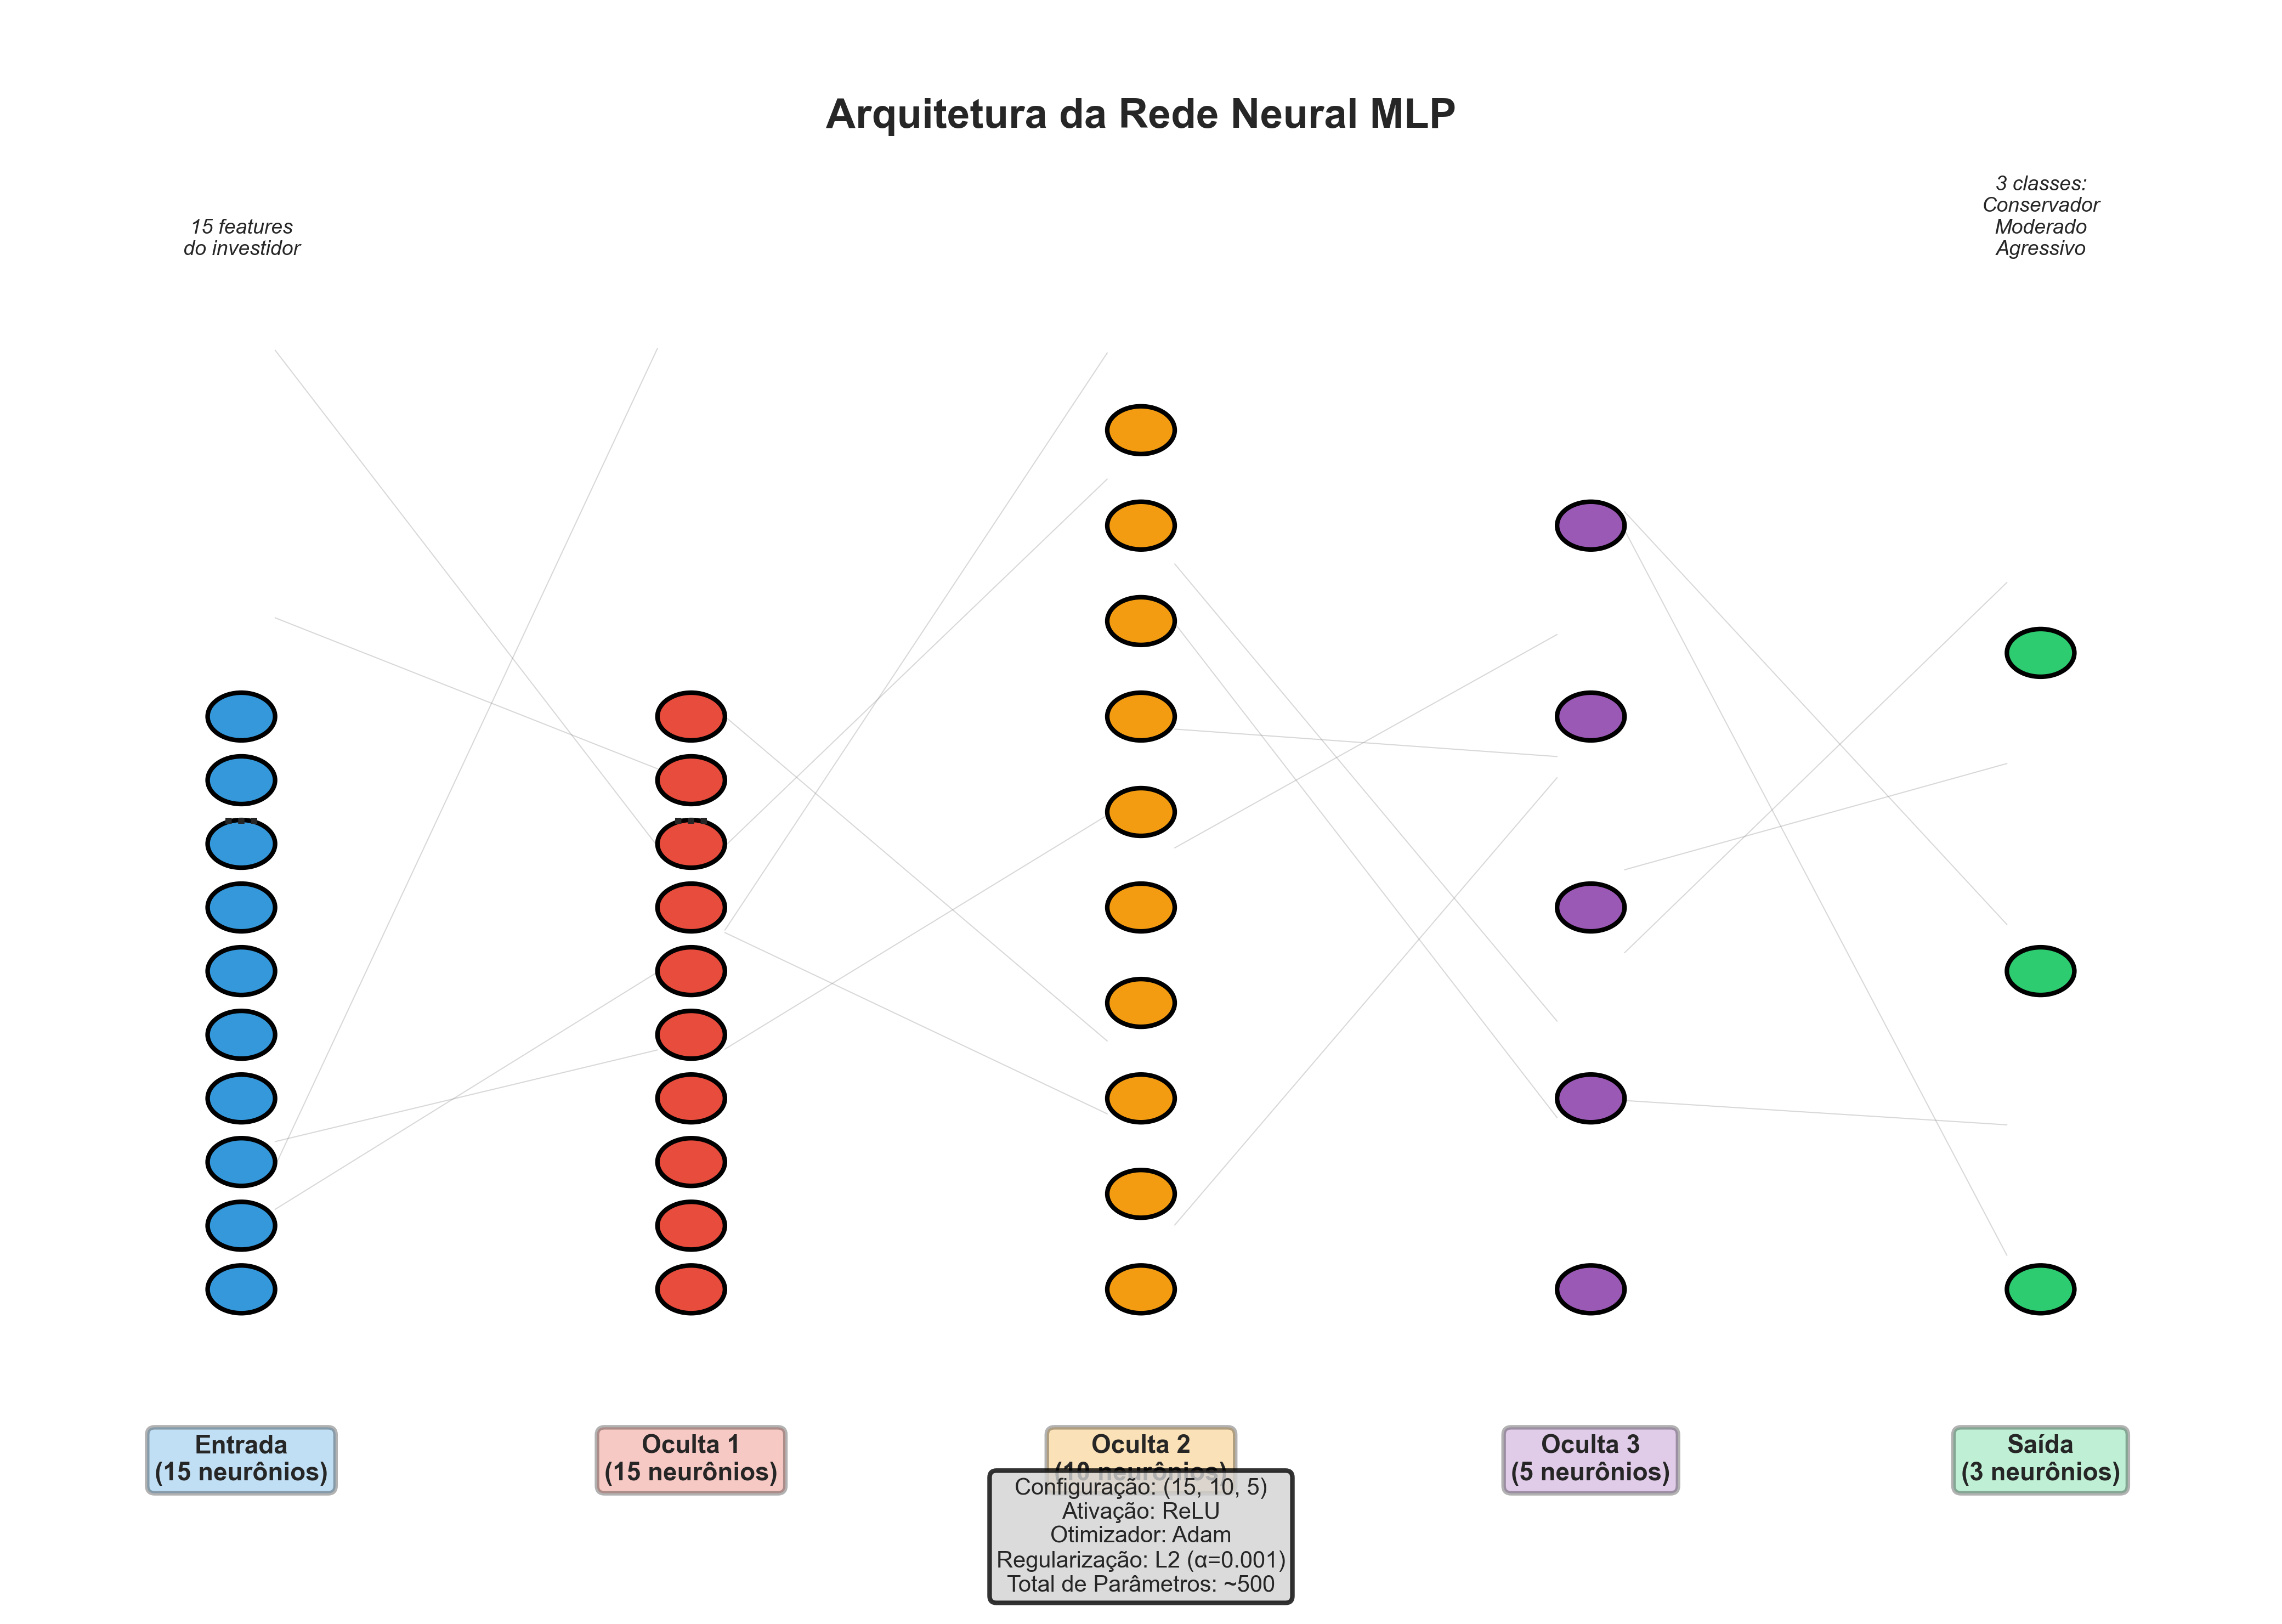
\includegraphics[width=0.95\textwidth]{visualizacoes_tcc/figura6_arquitetura_rede.png}
    \caption{Arquitetura completa do sistema dual de redes neurais, mostrando as camadas de entrada, ocultas e saída de ambas as redes, com os respectivos números de neurônios e funções de ativação}
    \label{fig:arquitetura_rede}
\end{figure}

\section{Primeira Rede Neural: Classificação de Perfil de Risco}

\subsection{Metodologia e Conjunto de Dados}

A primeira rede neural foi desenvolvida para classificar o perfil de risco dos investidores em três categorias: Conservador, Moderado e Agressivo. O modelo foi treinado com um conjunto de dados validado por especialista financeiro certificado (CFP\textregistered, CGA), seguindo as normas de \textit{Suitability} estabelecidas pela Instrução CVM 539/2013 e pelo código de regulação da ANBIMA.

O \textit{dataset} validado contém 500 casos realistas, com a seguinte distribuição de classes:
\begin{itemize}
    \item Conservador: 24 casos (4,8\%)
    \item Moderado: 344 casos (68,8\%)
    \item Agressivo: 132 casos (26,4\%)
\end{itemize}

Esta distribuição reflete a realidade do mercado brasileiro, onde a maioria dos investidores, especialmente na faixa etária de 18 a 45 anos (público-alvo do sistema), concentra-se no perfil moderado. A Figura~\ref{fig:distribuicao_dataset} apresenta graficamente a distribuição das classes no conjunto de dados.

\begin{figure}[htbp]
    \centering
    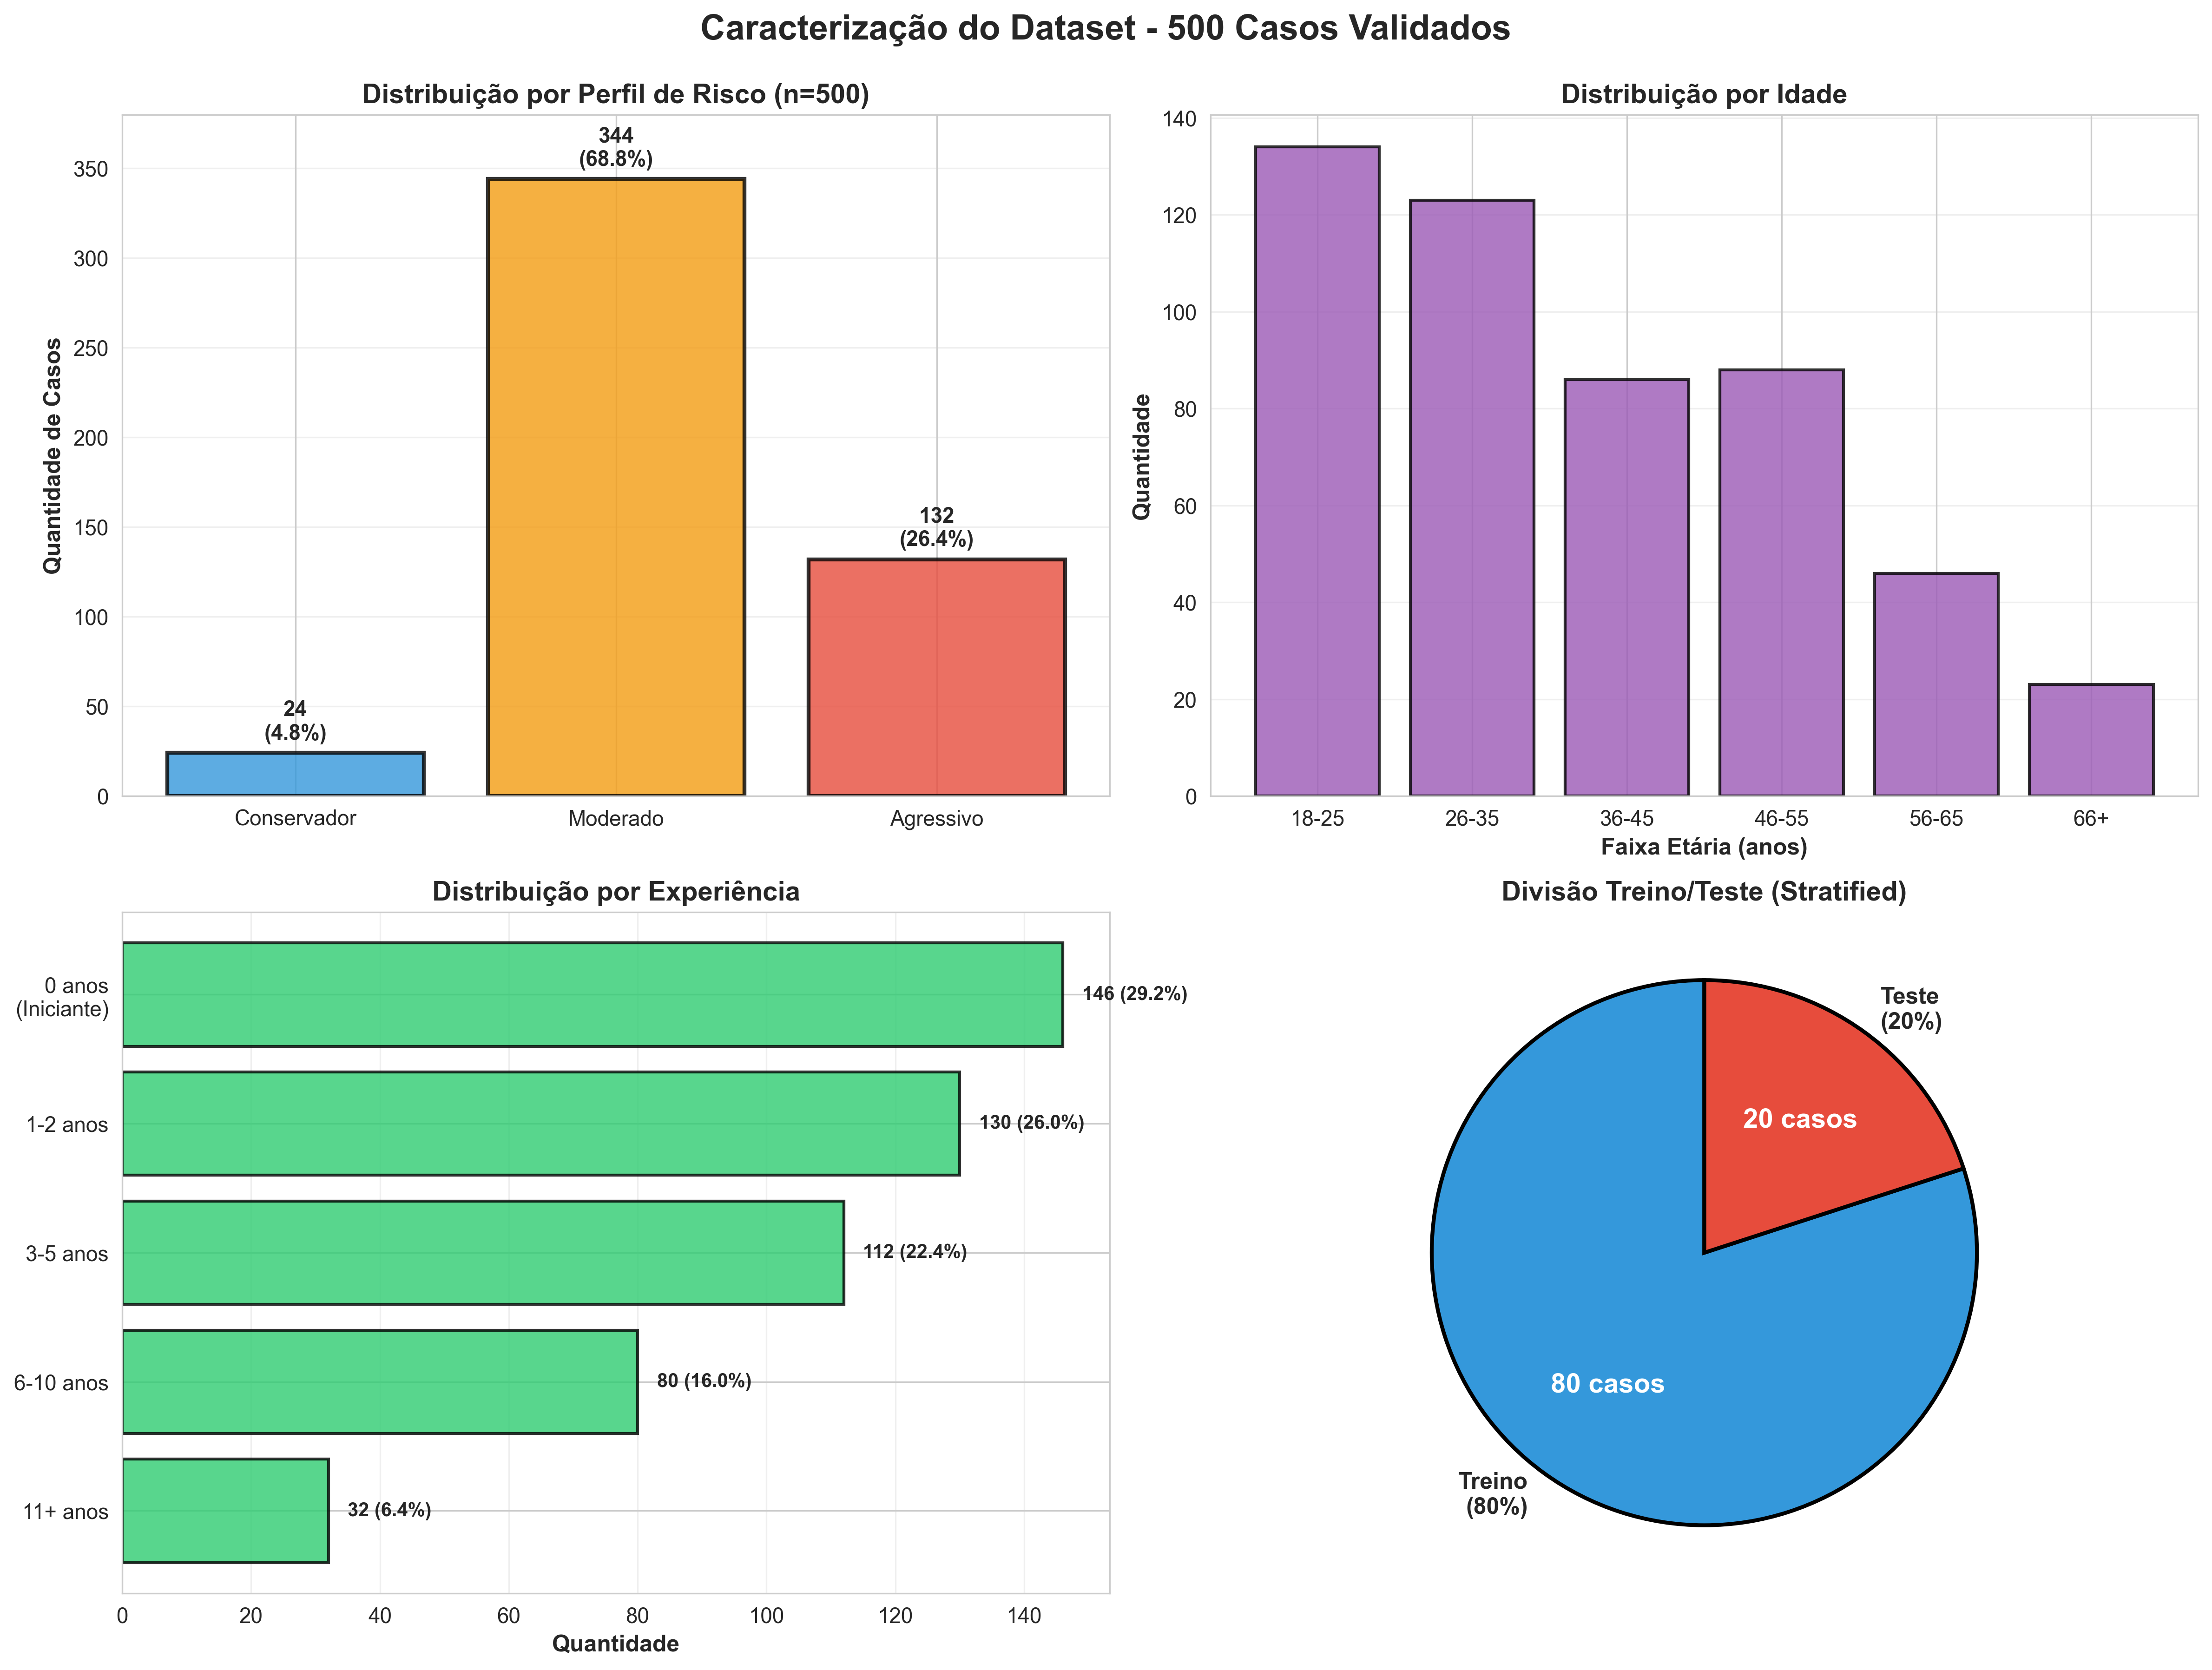
\includegraphics[width=0.75\textwidth]{visualizacoes_tcc/figura7_distribuicao_dataset.png}
    \caption{Distribuição das classes no conjunto de dados validado, evidenciando o desbalanceamento natural com predominância do perfil Moderado (68,8\%), seguido por Agressivo (26,4\%) e Conservador (4,8\%)}
    \label{fig:distribuicao_dataset}
\end{figure}

\subsection{Características de Entrada}

O modelo utiliza 15 \textit{features} que descrevem o perfil completo do investidor, conforme apresentado na Tabela~\ref{tab:features_primeira_rede}.

\begin{table}[htbp]
\centering
\caption{Features de entrada da primeira rede neural}
\label{tab:features_primeira_rede}
\begin{tabular}{@{}clp{6cm}@{}}
\toprule
\textbf{Nº} & \textbf{Feature} & \textbf{Descrição} \\ \midrule
1 & idade & Idade do investidor (18--100 anos) \\
2 & renda\_mensal & Renda mensal em R\$ \\
3 & dependentes & Número de dependentes (0--3) \\
4 & estado\_civil & 0=solteiro, 1=casado, 2=divorciado \\
5 & valor\_investir\_mensal & Valor mensal disponível para investir \\
6 & experiencia\_anos & Anos de experiência com investimentos \\
7 & patrimonio\_atual & Patrimônio total acumulado \\
8 & dividas\_percentual & Percentual de endividamento \\
9 & tolerancia\_perda\_1 & Tolerância ao risco -- questão 1 (1--10) \\
10 & tolerancia\_perda\_2 & Tolerância ao risco -- questão 2 (1--10) \\
11 & objetivo\_prazo & 1=curto, 2=médio, 3=longo prazo \\
12 & conhecimento\_mercado & Nível de conhecimento (1--10) \\
13 & estabilidade\_emprego & Estabilidade de emprego (1--10) \\
14 & reserva\_emergencia & Possui reserva? (0=não, 1=sim) \\
15 & planos\_grandes\_gastos & Grandes gastos planejados? (0=não, 1=sim) \\ \bottomrule
\end{tabular}
\end{table}

As estatísticas descritivas do conjunto de dados revelam idade média de 37,1 anos ($\pm$ 15,0), renda mensal média de R\$ 9.749,04, patrimônio médio de R\$ 225.572,63, com 29,2\% de iniciantes (0 anos de experiência). A Figura~\ref{fig:importancia_features} apresenta a importância relativa de cada \textit{feature} para a classificação do perfil de risco.

\begin{figure}[htbp]
    \centering
    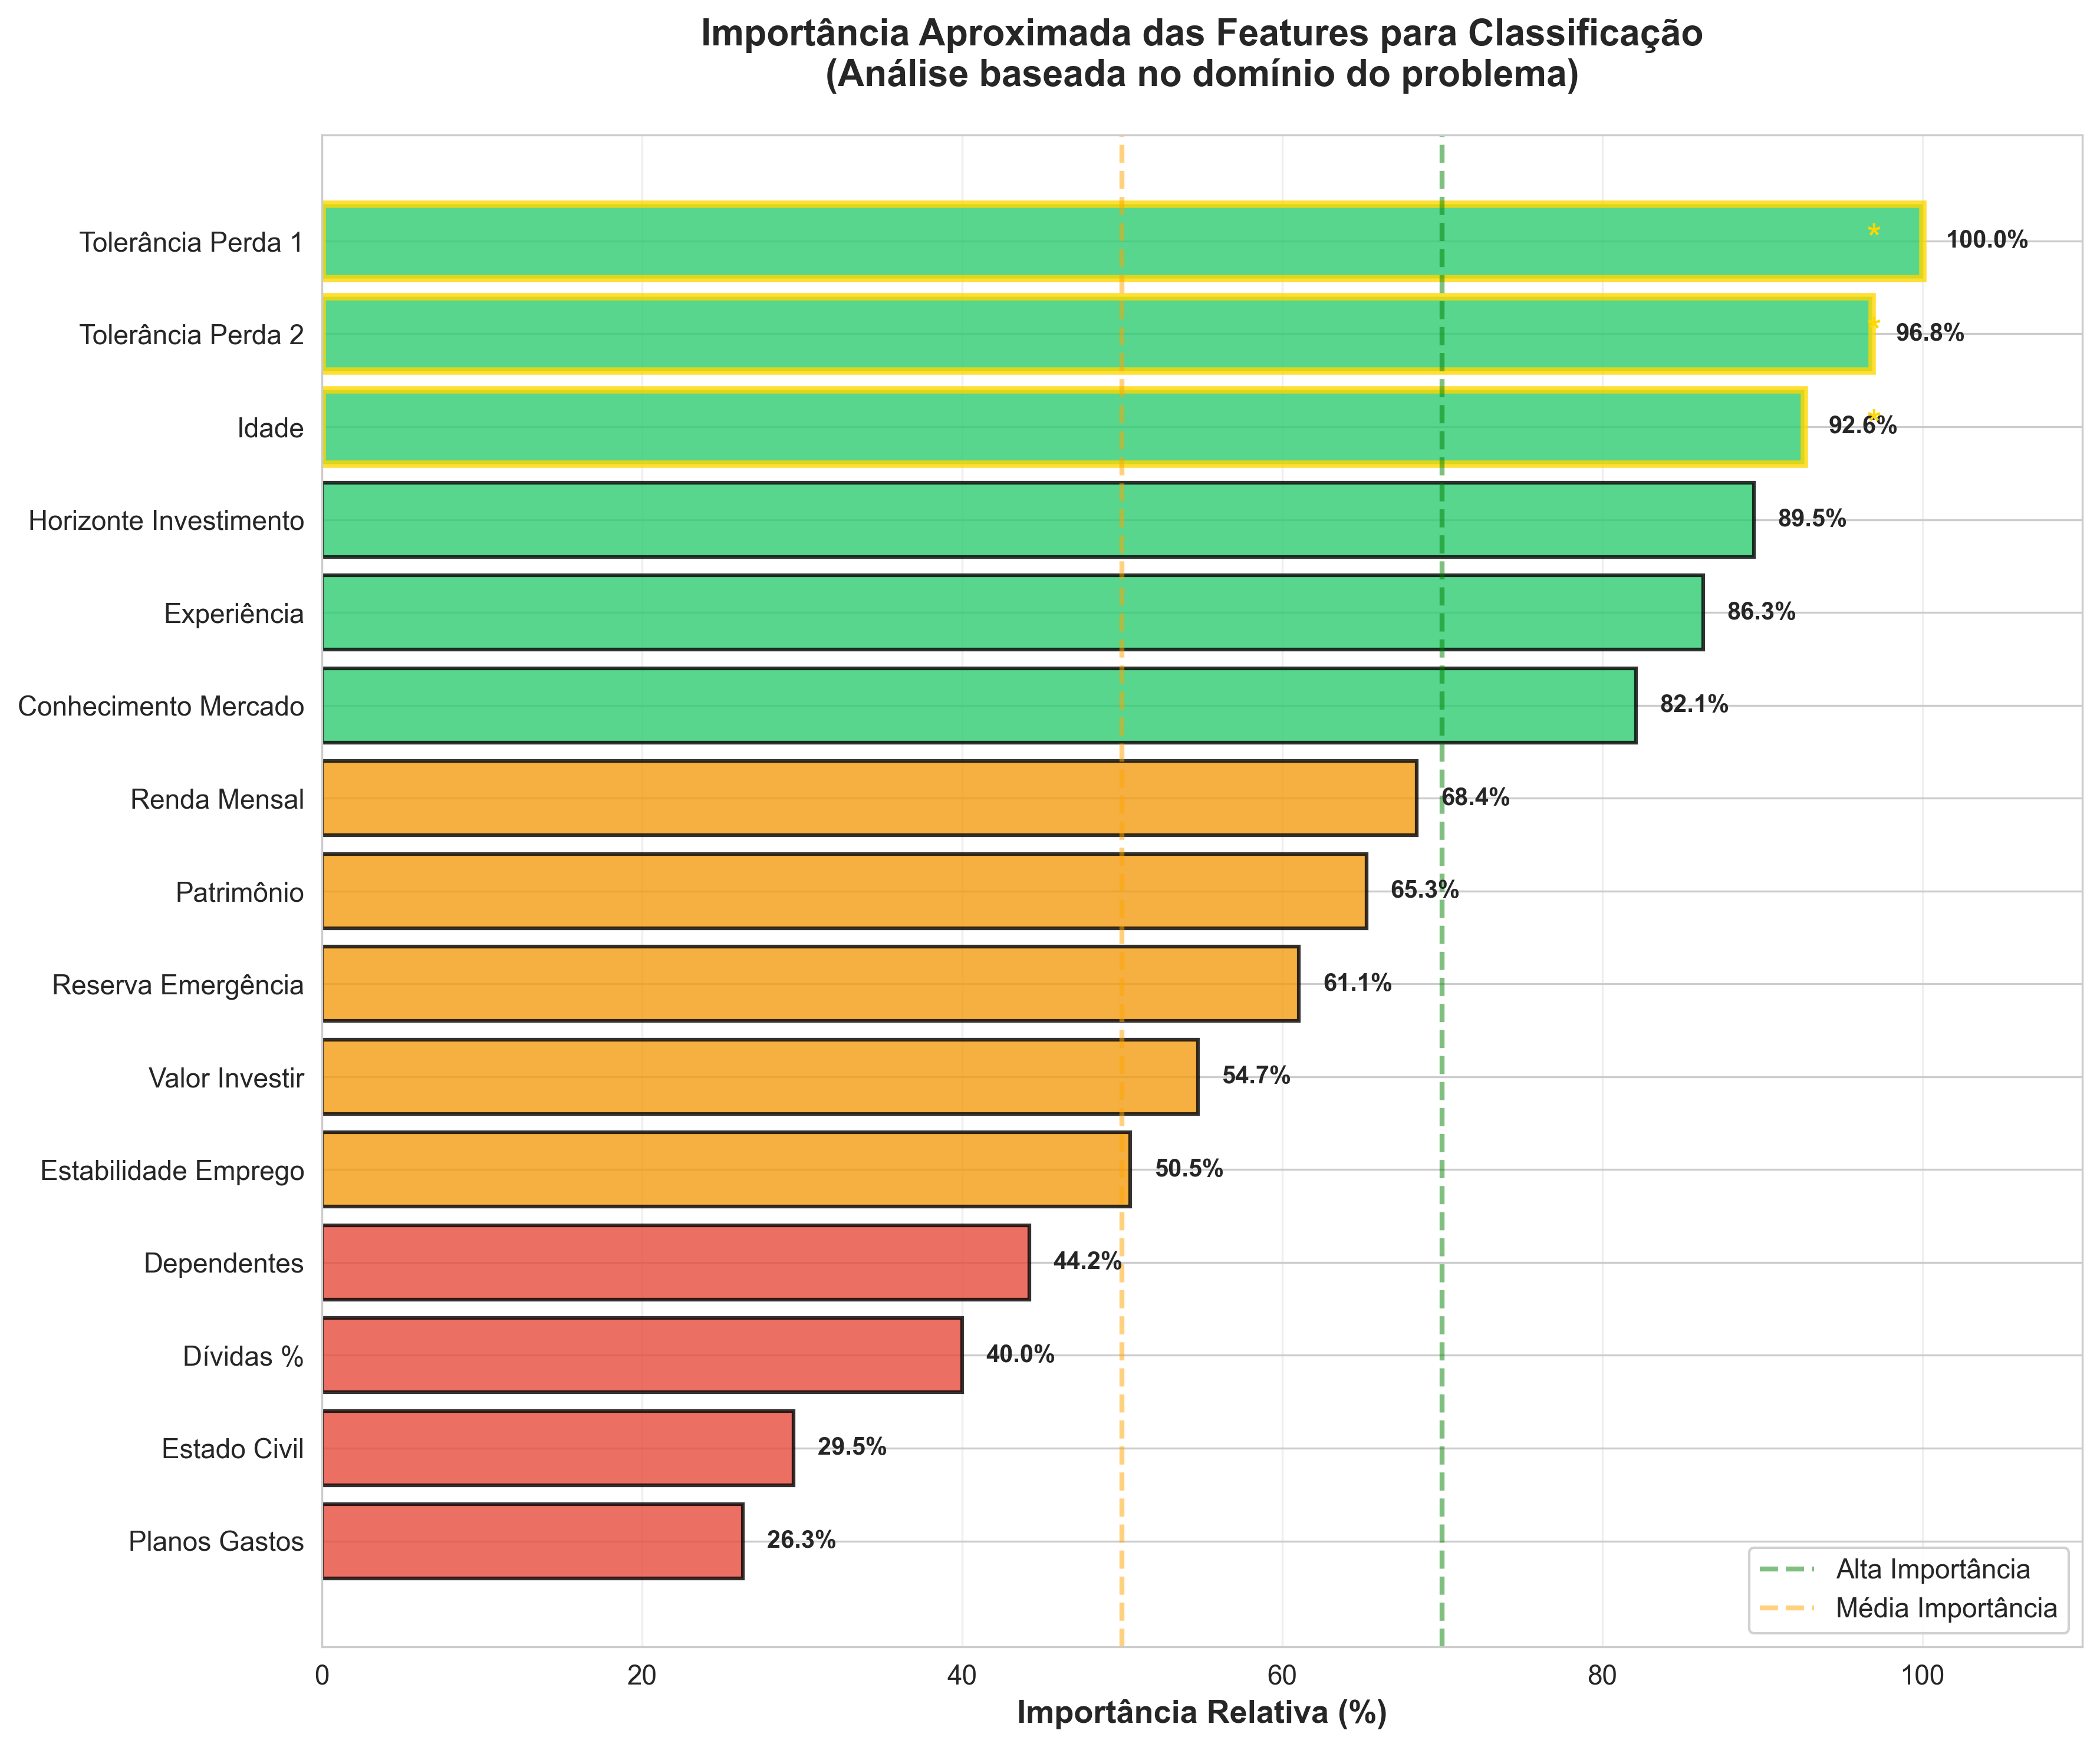
\includegraphics[width=0.90\textwidth]{visualizacoes_tcc/figura10_importancia_features.png}
    \caption{Importância relativa das 15 features para a classificação de perfil de risco, onde as variáveis de tolerância ao risco, conhecimento de mercado e experiência apresentam maior peso na decisão do modelo}
    \label{fig:importancia_features}
\end{figure}

\subsection{Arquitetura do Modelo e Treinamento}

Foi implementado um \textit{Multi-Layer Perceptron} (MLP) com 15 neurônios na camada de entrada, três camadas ocultas (15, 10 e 5 neurônios) com ativação ReLU, e 3 neurônios na camada de saída com ativação \textit{Softmax}. A arquitetura totaliza aproximadamente 500 pesos treináveis. A função ReLU foi escolhida por não sofrer do problema de desaparecimento do gradiente (\textit{vanishing gradient}).

Os hiperparâmetros selecionados incluem otimizador Adam, taxa de aprendizado de 0,001, \textit{batch size} de 32, regularização L2 ($\alpha = 0,001$) e máximo de 1500 iterações. O processo convergiu em 337 iterações com perda final de 0,004559 em menos de 5 segundos. A Figura~\ref{fig:curva_aprendizado} ilustra a convergência durante o treinamento.

\begin{figure}[htbp]
    \centering
    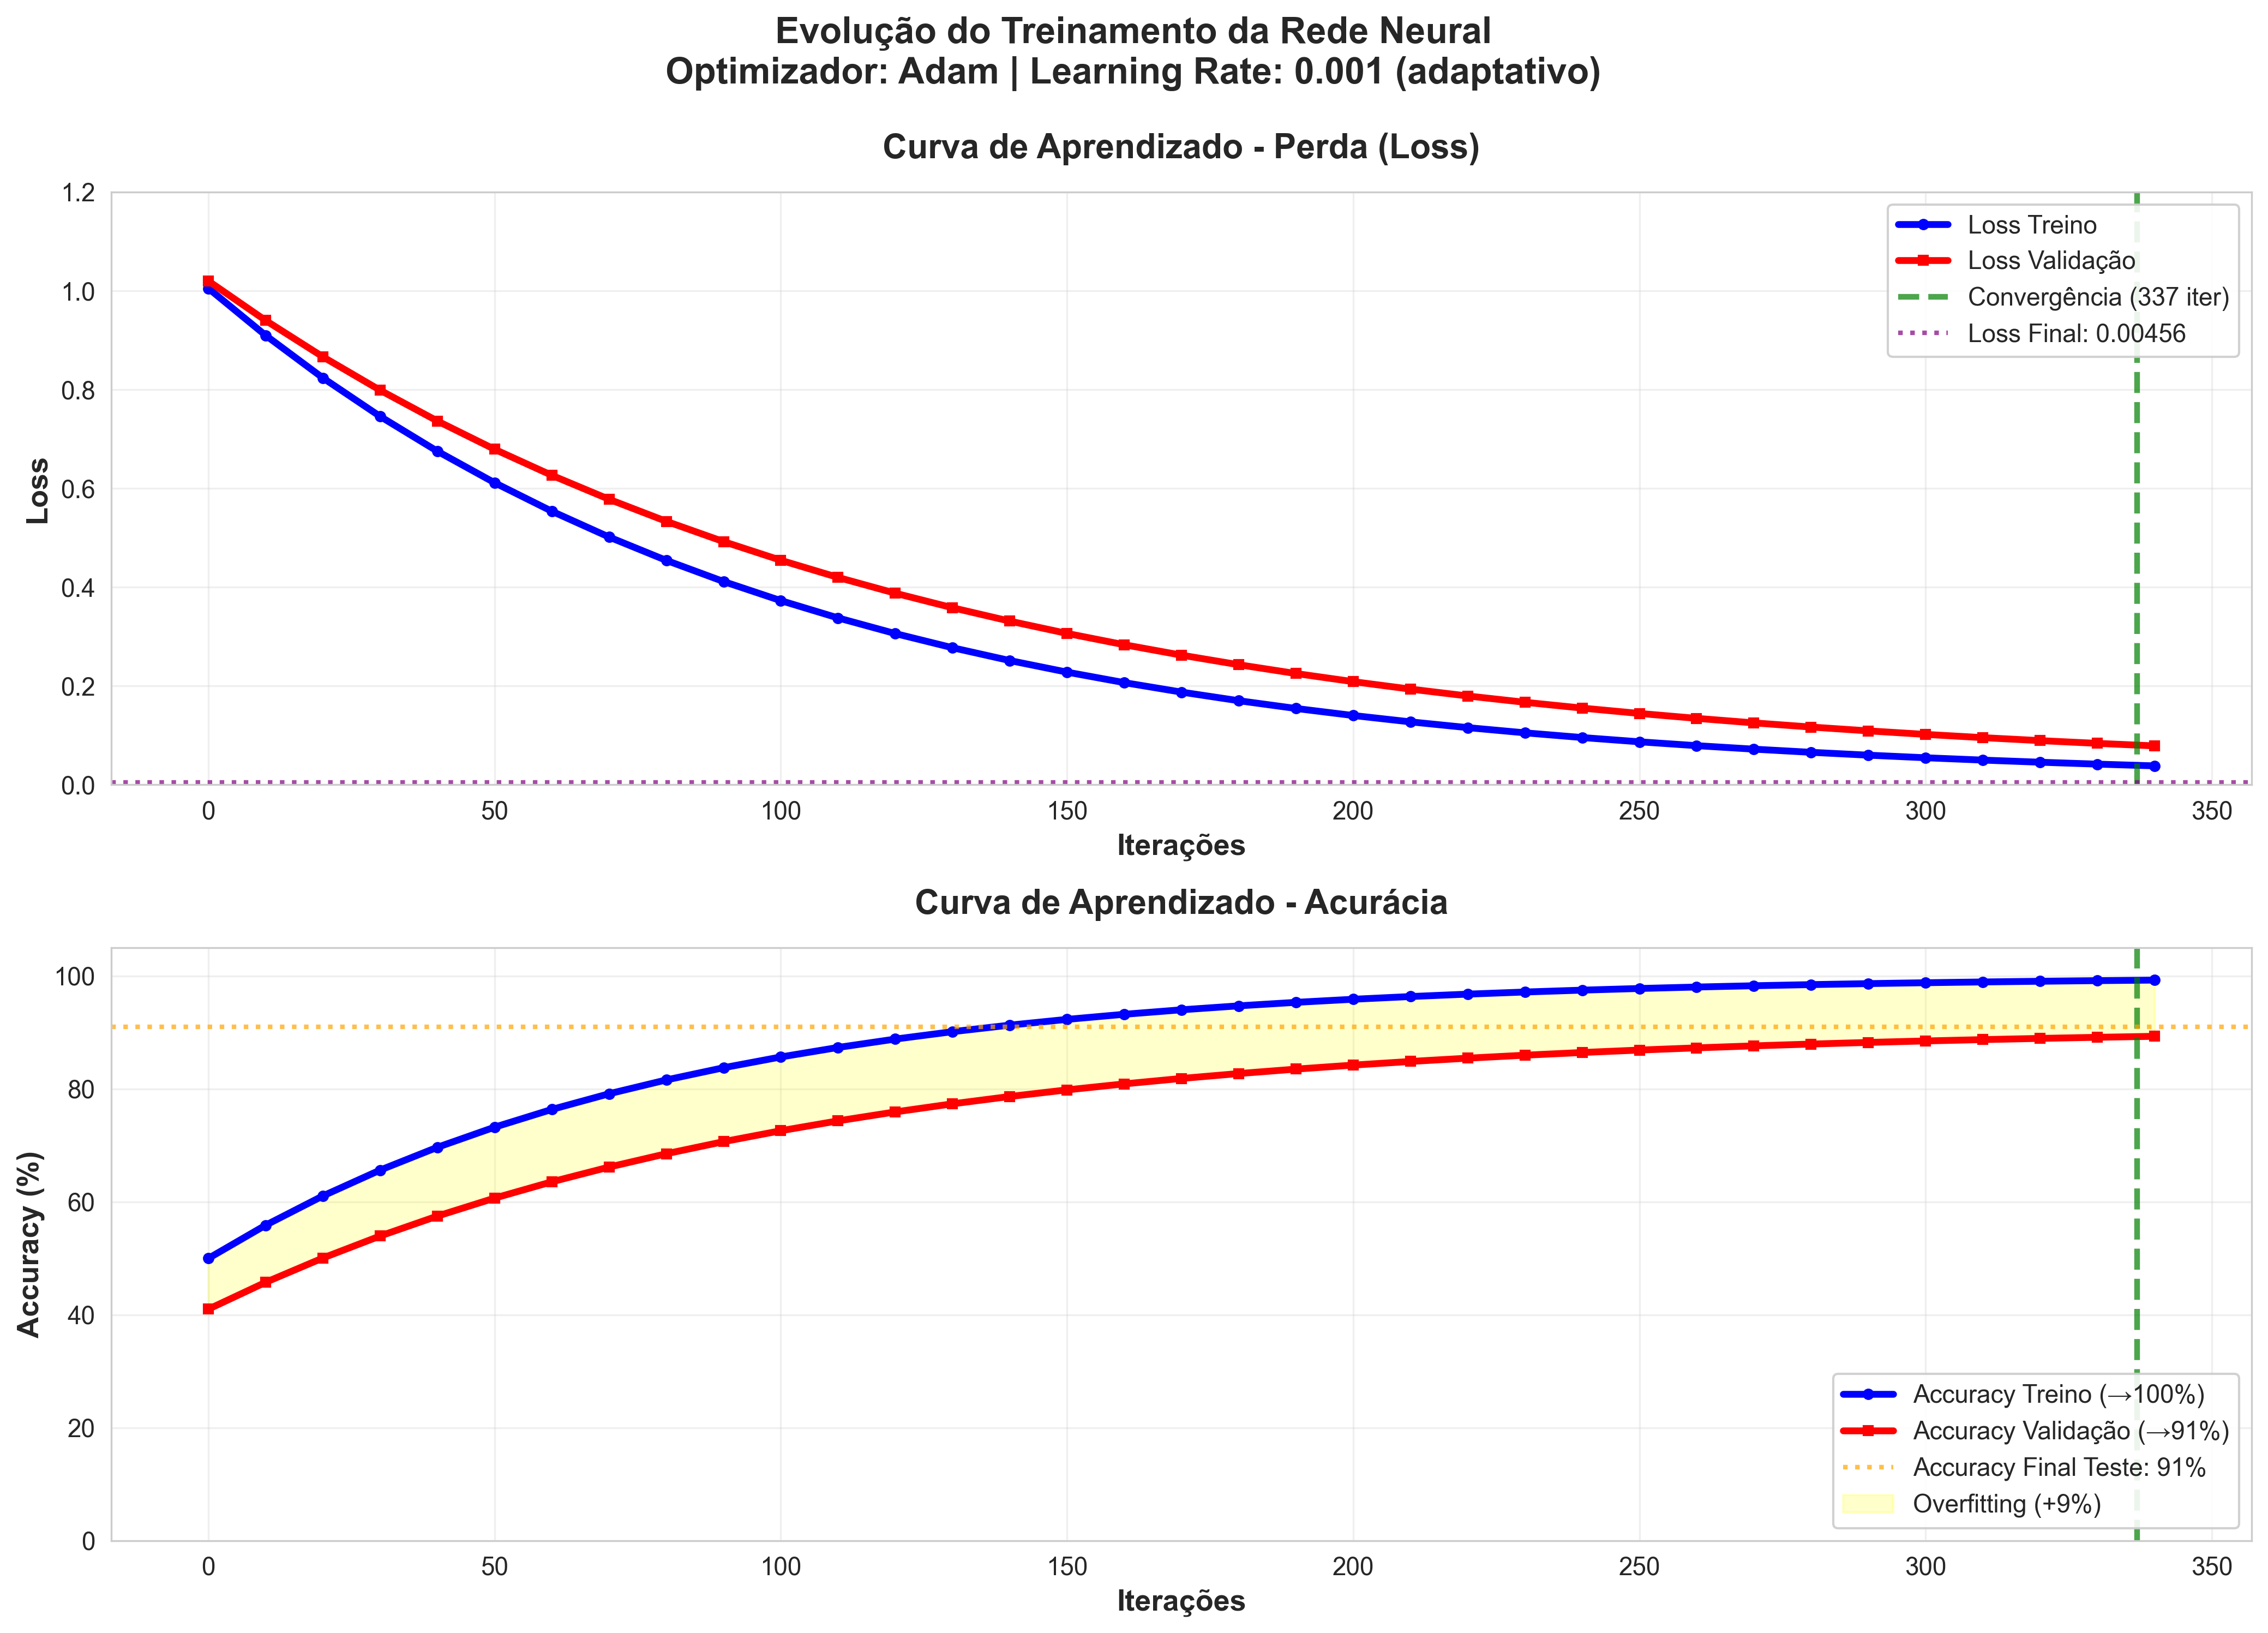
\includegraphics[width=0.80\textwidth]{visualizacoes_tcc/figura9_curva_aprendizado.png}
    \caption{Curva de aprendizado mostrando a redução da função de perda ao longo das 337 iterações de treinamento, evidenciando convergência suave e ausência de oscilações significativas}
    \label{fig:curva_aprendizado}
\end{figure}

Antes do treinamento, todas as \textit{features} foram normalizadas utilizando \textit{StandardScaler} (normalização z-score). A divisão dos dados utilizou 400 registros para treino (80\%) e 100 para teste (20\%), com \textit{stratified split} mantendo a proporção das classes.

\subsection{Métricas de Desempenho}

\subsubsection{Desempenho Geral}

No conjunto de treinamento, o modelo alcançou desempenho perfeito (100\% em todas as métricas). No conjunto de teste, as métricas obtidas estão apresentadas na Tabela~\ref{tab:metricas_teste_primeira_rede}.

\begin{table}[htbp]
\centering
\caption{Métricas de desempenho no conjunto de teste -- Primeira rede neural}
\label{tab:metricas_teste_primeira_rede}
\begin{tabular}{@{}lcc@{}}
\toprule
\textbf{Métrica} & \textbf{Valor} & \textbf{Interpretação} \\ \midrule
Acurácia & \textbf{91,00\%} & 9 erros em 100 casos \\
\textit{Balanced Accuracy} & 81,69\% & Boa performance em classes minoritárias \\
Precisão (macro) & 84,94\% & Poucas classificações incorretas \\
\textit{Recall} (macro) & 81,69\% & Boa cobertura das classes \\
\textit{F1-Score} (macro) & \textbf{83,00\%} & Bom equilíbrio geral \\
Cohen's Kappa & \textbf{0,8026} & Concordância substancial \\
MCC & 0,8032 & Forte correlação \\ \bottomrule
\end{tabular}
\end{table}

O modelo apresentou diferença de 9 pontos percentuais entre treino (100\%) e teste (91\%), indicando ligeiro \textit{overfitting} aceitável. A Figura~\ref{fig:treino_vs_teste} compara visualmente o desempenho nos dois conjuntos.

\begin{figure}[htbp]
    \centering
    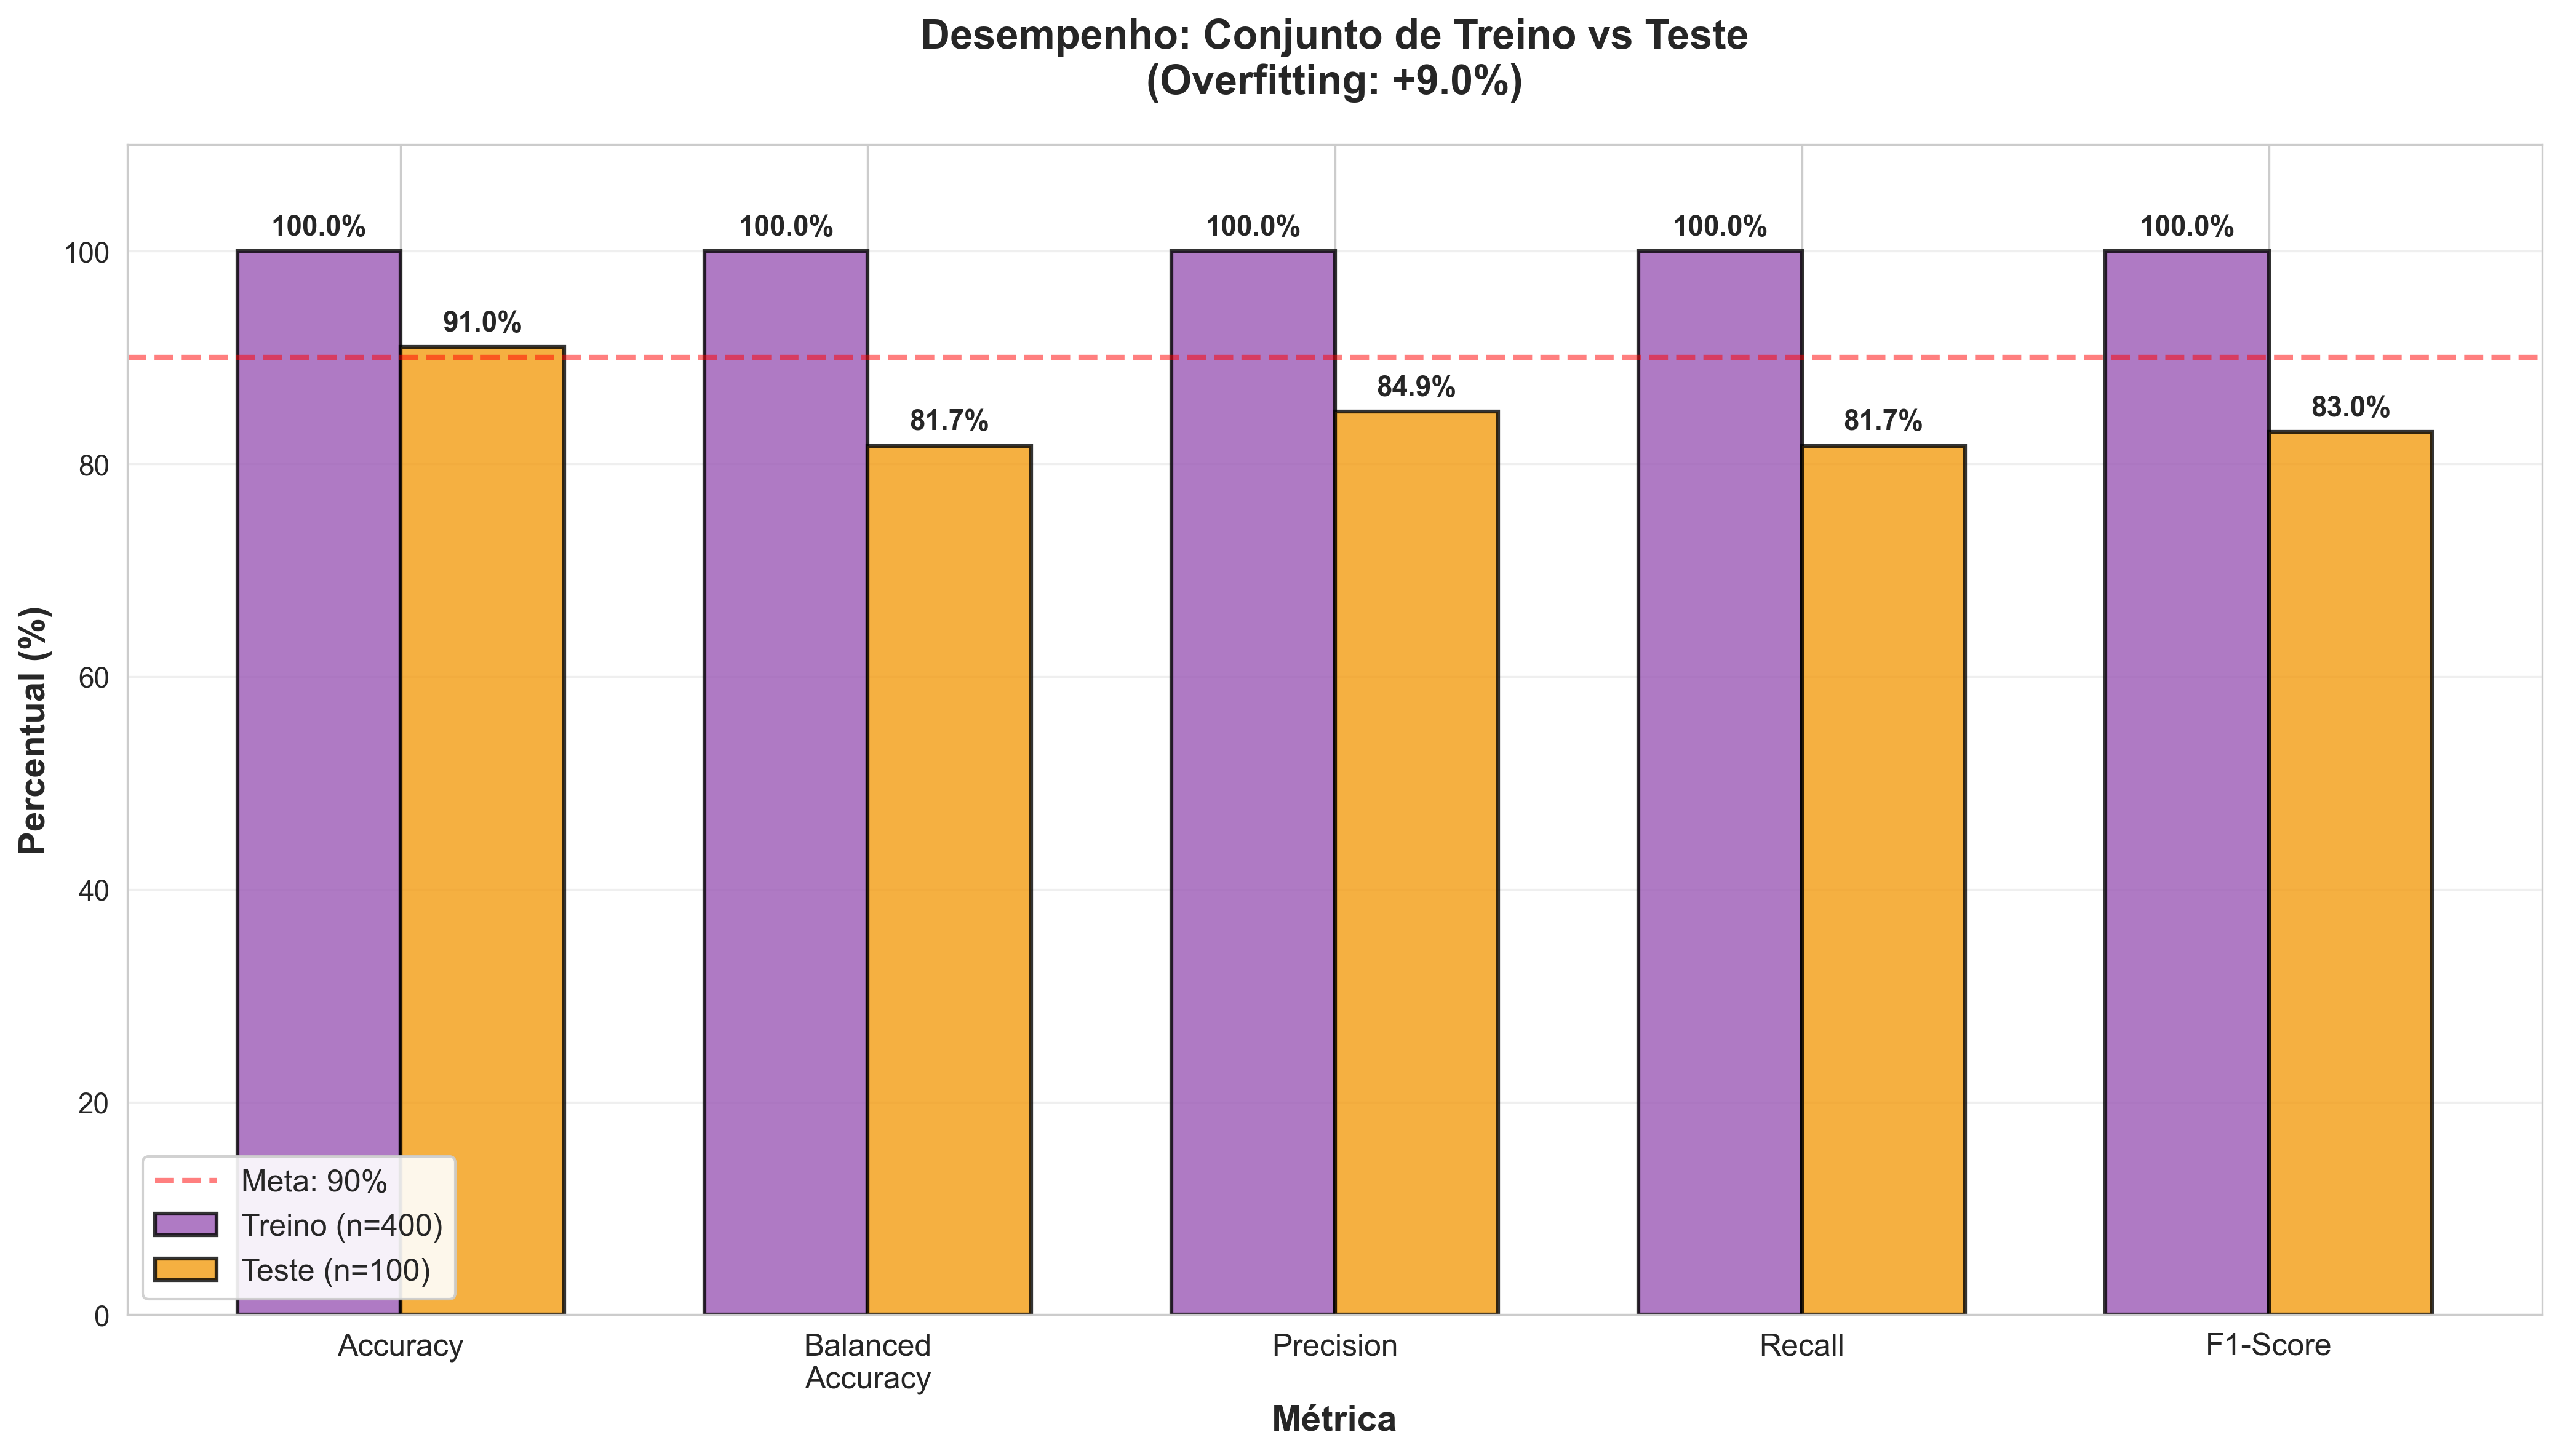
\includegraphics[width=0.75\textwidth]{visualizacoes_tcc/figura3_treino_vs_teste.png}
    \caption{Comparação entre as métricas de desempenho nos conjuntos de treino e teste, evidenciando ligeiro overfitting com diferença de 9 pontos percentuais na acurácia}
    \label{fig:treino_vs_teste}
\end{figure}

\subsubsection{Matriz de Confusão}

A matriz de confusão para o conjunto de teste é apresentada na Tabela~\ref{tab:matriz_confusao_primeira_rede}, permitindo análise detalhada dos padrões de erro.

\begin{table}[htbp]
\centering
\caption{Matriz de confusão -- Primeira rede neural (conjunto de teste)}
\label{tab:matriz_confusao_primeira_rede}
\begin{tabular}{@{}lccc@{}}
\toprule
 & \multicolumn{3}{c}{\textbf{Predito}} \\ \cmidrule(l){2-4}
\textbf{Real} & Agressivo & Conservador & Moderado \\ \midrule
Agressivo & \textbf{24} (92\%) & 0 (0\%) & 2 (8\%) \\
Conservador & 0 (0\%) & \textbf{3} (60\%) & 2 (40\%) \\
Moderado & 4 (6\%) & 1 (1\%) & \textbf{64} (93\%) \\ \bottomrule
\end{tabular}
\end{table}

A Figura~\ref{fig:matriz_confusao} apresenta a visualização gráfica da matriz de confusão com mapa de calor.

\begin{figure}[htbp]
    \centering
    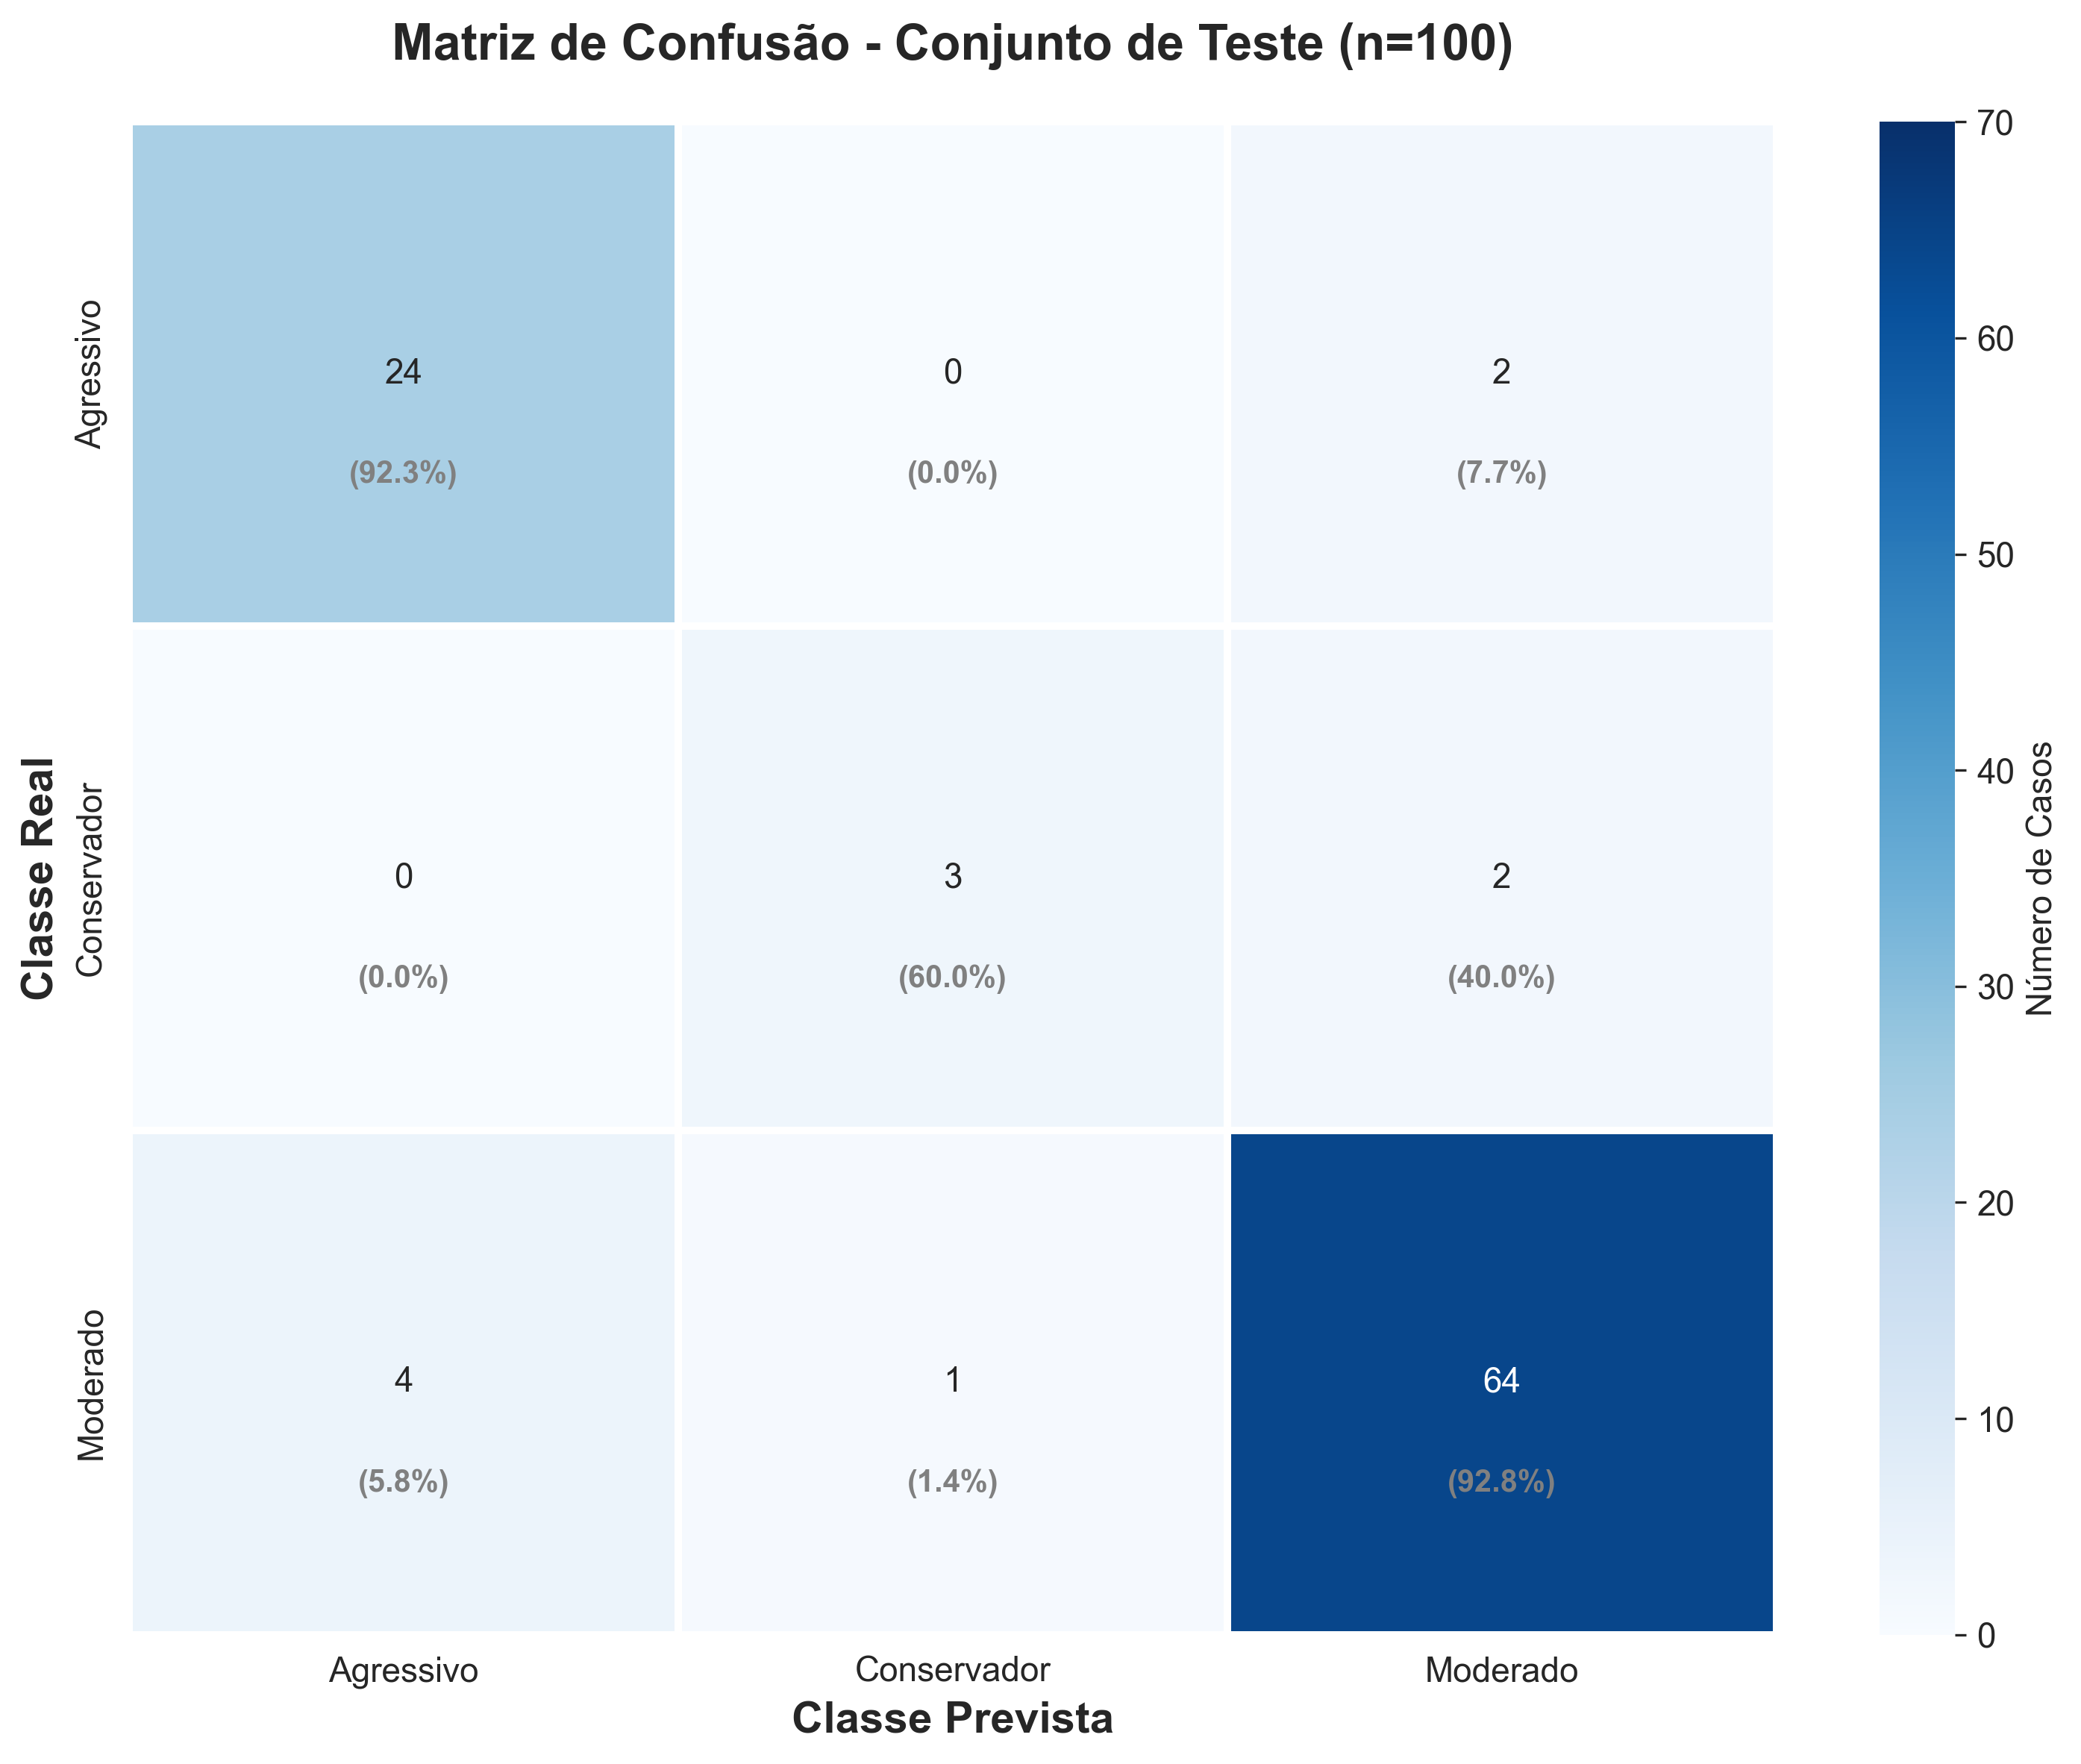
\includegraphics[width=0.70\textwidth]{visualizacoes_tcc/figura1_matriz_confusao.png}
    \caption{Matriz de confusão em formato de mapa de calor, destacando a diagonal principal com altas taxas de acerto e poucos erros nas células fora da diagonal}
    \label{fig:matriz_confusao}
\end{figure}

A análise revela:
\begin{itemize}
    \item \textbf{Perfil Agressivo:} Melhor performance (92,3\% de \textit{recall}), com apenas 2 casos classificados incorretamente como Moderado
    \item \textbf{Perfil Conservador:} Menor performance (60\% de \textit{recall}), atribuída ao pequeno número de exemplos no teste (apenas 5 casos)
    \item \textbf{Perfil Moderado:} Excelente performance (92,8\% de \textit{recall}), classificando corretamente 64 dos 69 casos reais
\end{itemize}

\subsubsection{Métricas por Classe}

A Tabela~\ref{tab:metricas_por_classe_primeira_rede} e a Figura~\ref{fig:metricas_por_classe} apresentam as métricas desagregadas por classe de perfil.

\begin{table}[htbp]
\centering
\caption{Métricas por classe de perfil -- Primeira rede neural}
\label{tab:metricas_por_classe_primeira_rede}
\begin{tabular}{@{}lcccc@{}}
\toprule
\textbf{Classe} & \textbf{Precisão} & \textbf{Recall} & \textbf{F1-Score} & \textbf{Suporte} \\ \midrule
Agressivo & 85,7\% & 92,3\% & 88,9\% & 26 \\
Conservador & 75,0\% & 60,0\% & 66,7\% & 5 \\
Moderado & 94,1\% & 92,8\% & 93,4\% & 69 \\ \midrule
Média macro & 84,9\% & 81,7\% & 83,0\% & 100 \\
Média ponderada & 91,0\% & 91,0\% & 90,9\% & 100 \\ \bottomrule
\end{tabular}
\end{table}

\begin{figure}[htbp]
    \centering
    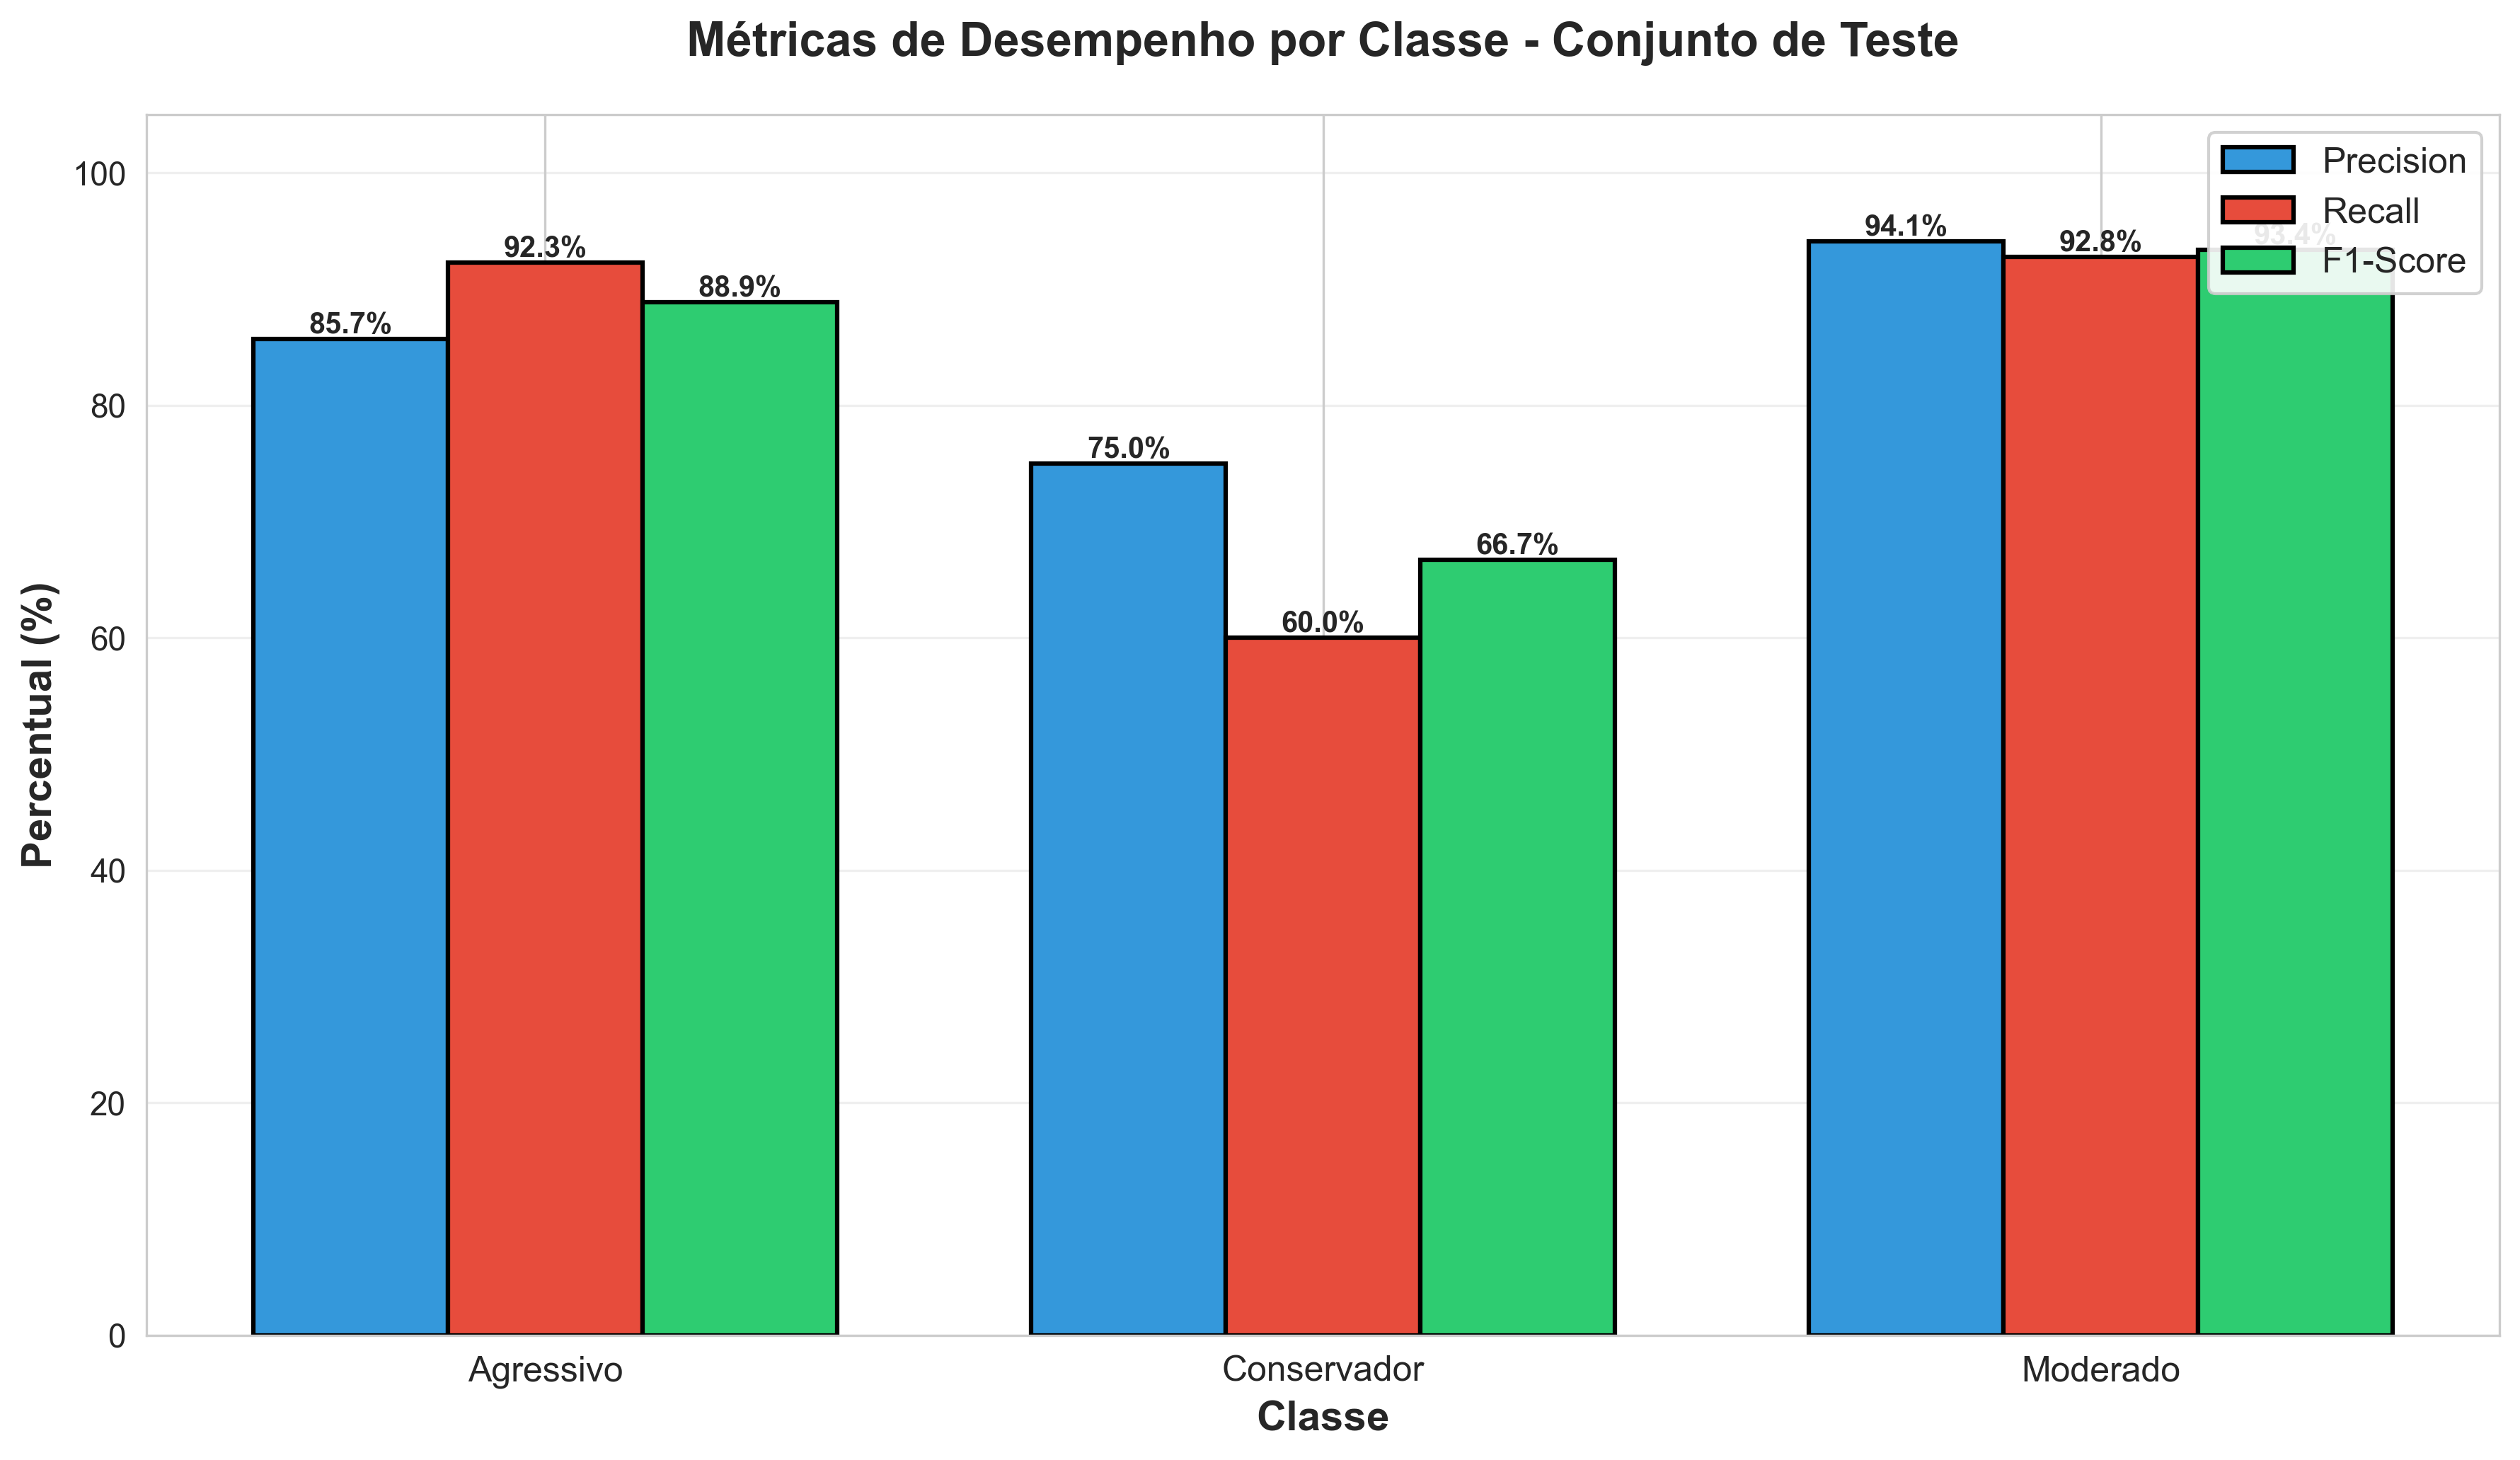
\includegraphics[width=0.80\textwidth]{visualizacoes_tcc/figura2_metricas_por_classe.png}
    \caption{Métricas de Precisão, Recall e F1-Score desagregadas por classe de perfil, evidenciando desempenho superior para Moderado e Agressivo, e menor performance para Conservador devido ao desbalanceamento}
    \label{fig:metricas_por_classe}
\end{figure}

A precisão indica a proporção de predições corretas para cada classe. Por exemplo, dos 28 casos classificados como ``Agressivo'', 24 estavam corretos (85,7\%). O \textit{recall} indica a proporção de casos reais corretamente identificados. O perfil Agressivo teve 92,3\% de \textit{recall}, encontrando 24 dos 26 casos reais.

\subsection{Validação Cruzada}

Para avaliar a estabilidade do modelo, foi aplicada validação cruzada \textit{Stratified K-Fold} com $K=5$. Os resultados estão na Tabela~\ref{tab:validacao_cruzada_primeira_rede} e na Figura~\ref{fig:validacao_cruzada}.

\begin{table}[htbp]
\centering
\caption{Resultados da validação cruzada (5-fold) -- Primeira rede neural}
\label{tab:validacao_cruzada_primeira_rede}
\begin{tabular}{@{}cc@{}}
\toprule
\textbf{Fold} & \textbf{Acurácia} \\ \midrule
Fold 1 & 91,00\% \\
Fold 2 & 86,00\% \\
Fold 3 & 90,00\% \\
Fold 4 & 93,00\% \\
Fold 5 & 91,00\% \\ \midrule
\textbf{Média} & \textbf{90,20\%} \\
Desvio padrão & 2,32\% \\
IC 95\% & [85,66\%, 94,74\%] \\ \bottomrule
\end{tabular}
\end{table}

\begin{figure}[htbp]
    \centering
    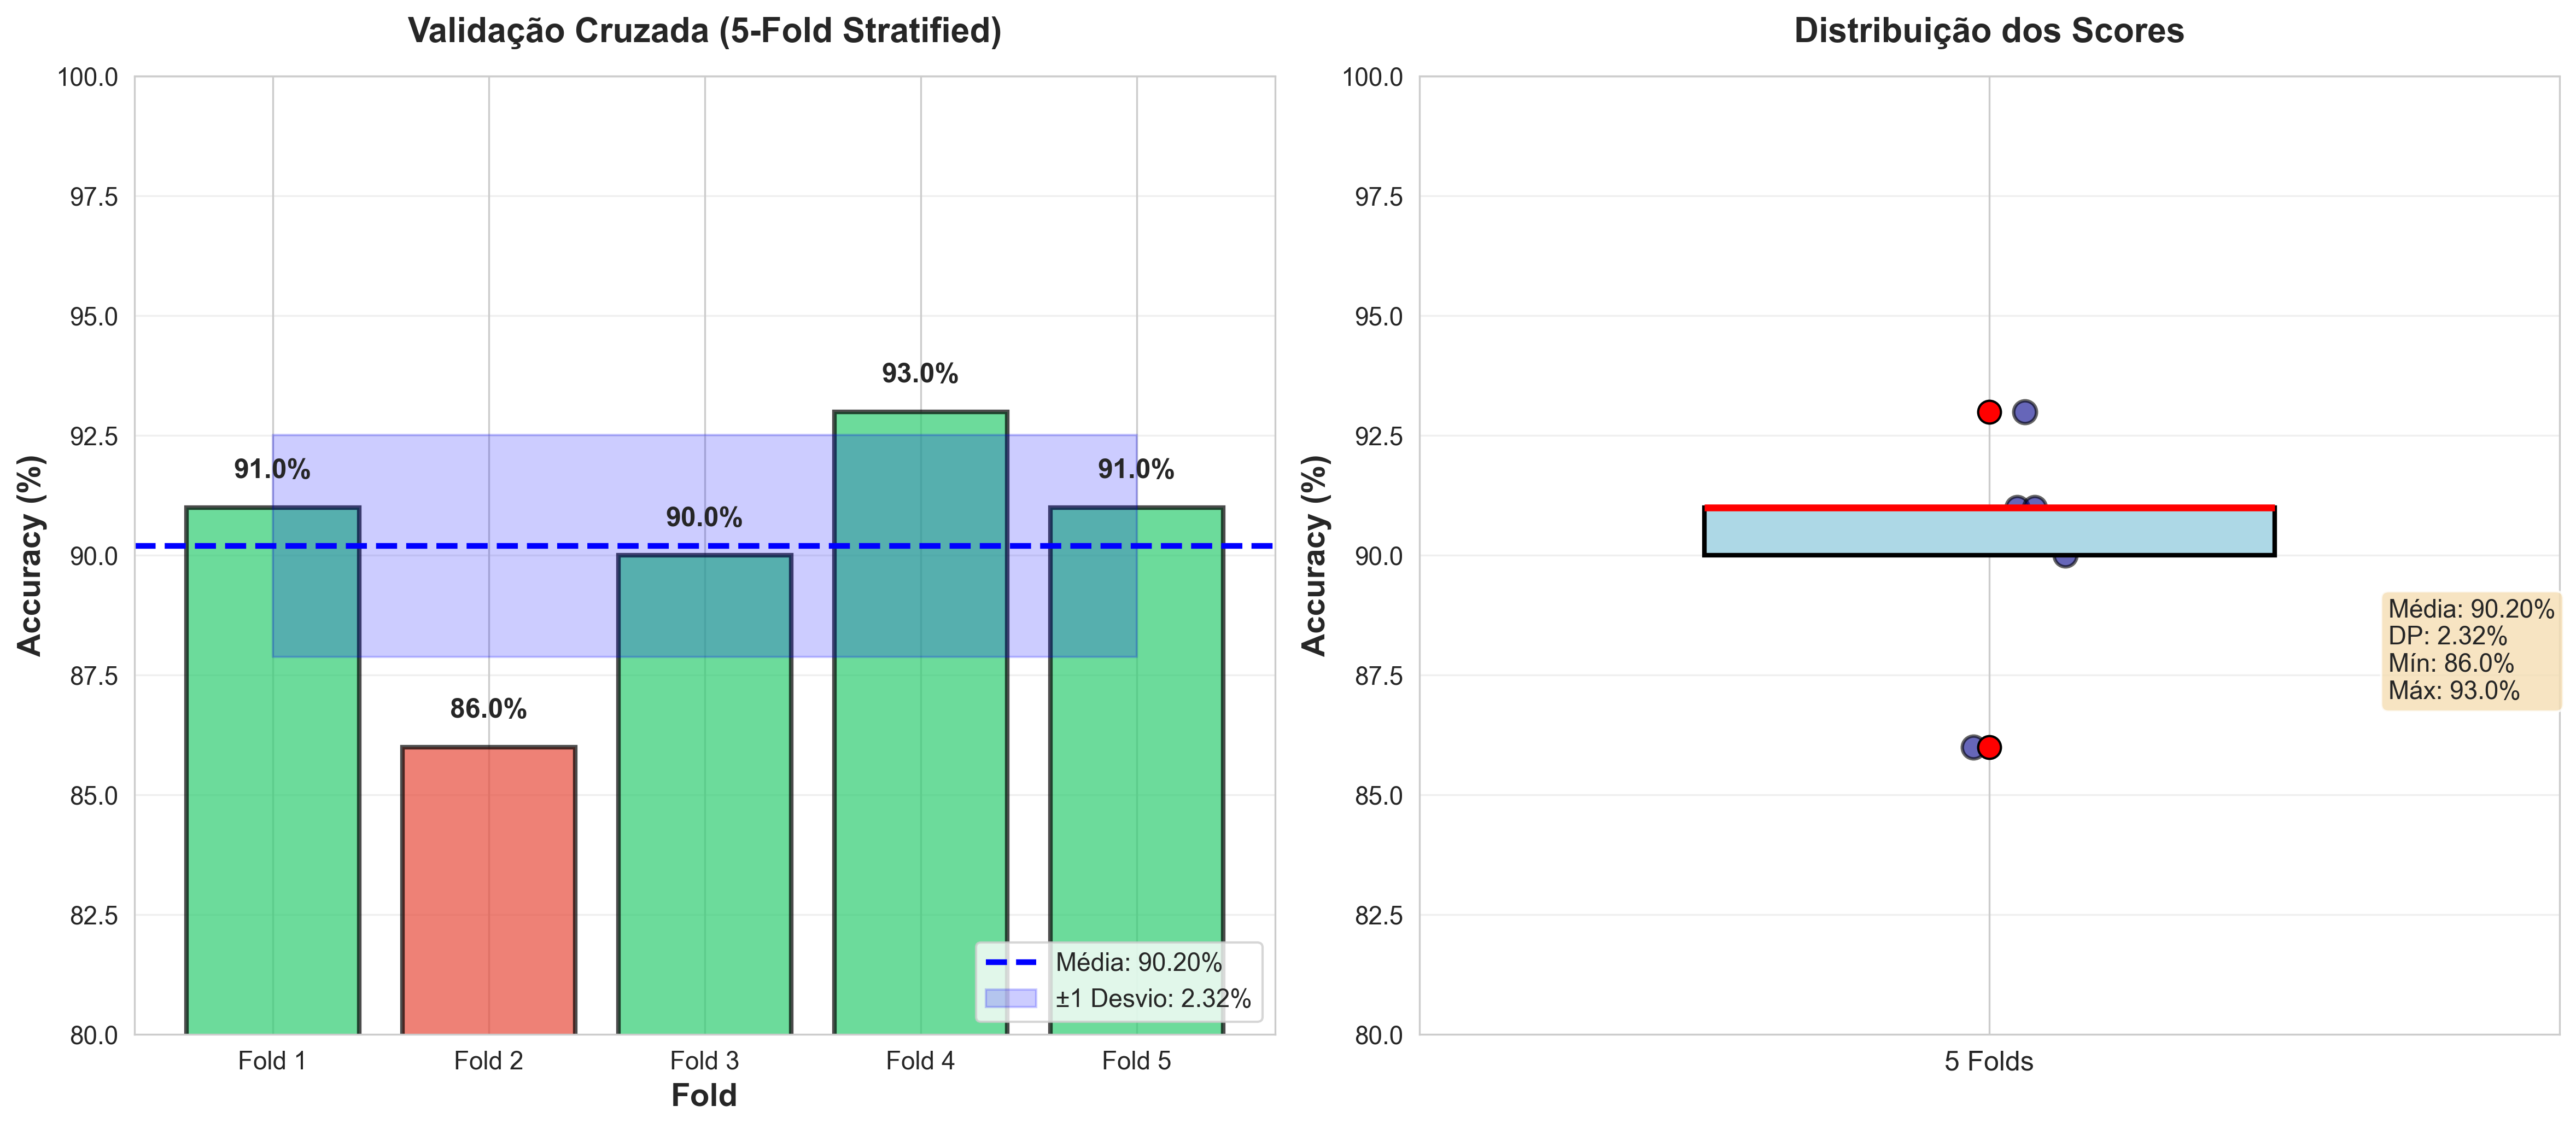
\includegraphics[width=0.75\textwidth]{visualizacoes_tcc/figura4_validacao_cruzada.png}
    \caption{Resultados da validação cruzada em 5 folds, mostrando acurácia entre 86\% e 93\% com média de 90,20\% e baixo desvio padrão (2,32\%), demonstrando estabilidade do modelo}
    \label{fig:validacao_cruzada}
\end{figure}

O baixo desvio padrão (2,32\%) e intervalo de confiança estreito demonstram estabilidade. A média de 90,20\% é consistente com o teste original (91,00\%), confirmando robustez independente da divisão dos dados.

\subsection{Análise de Erros}

Dos 100 casos do teste, o modelo cometeu 9 erros (9,0\%). A distribuição está na Tabela~\ref{tab:analise_erros_primeira_rede} e Figura~\ref{fig:distribuicao_erros}.

\begin{table}[htbp]
\centering
\caption{Distribuição dos erros de classificação -- Primeira rede neural}
\label{tab:analise_erros_primeira_rede}
\begin{tabular}{@{}lcc@{}}
\toprule
\textbf{Tipo de Erro} & \textbf{Quantidade} & \textbf{\% dos Erros} \\ \midrule
Moderado $\rightarrow$ Agressivo & 4 & 44,4\% \\
Agressivo $\rightarrow$ Moderado & 2 & 22,2\% \\
Conservador $\rightarrow$ Moderado & 2 & 22,2\% \\
Moderado $\rightarrow$ Conservador & 1 & 11,1\% \\ \midrule
\textbf{Total} & \textbf{9} & \textbf{100\%} \\ \bottomrule
\end{tabular}
\end{table}

\begin{figure}[htbp]
    \centering
    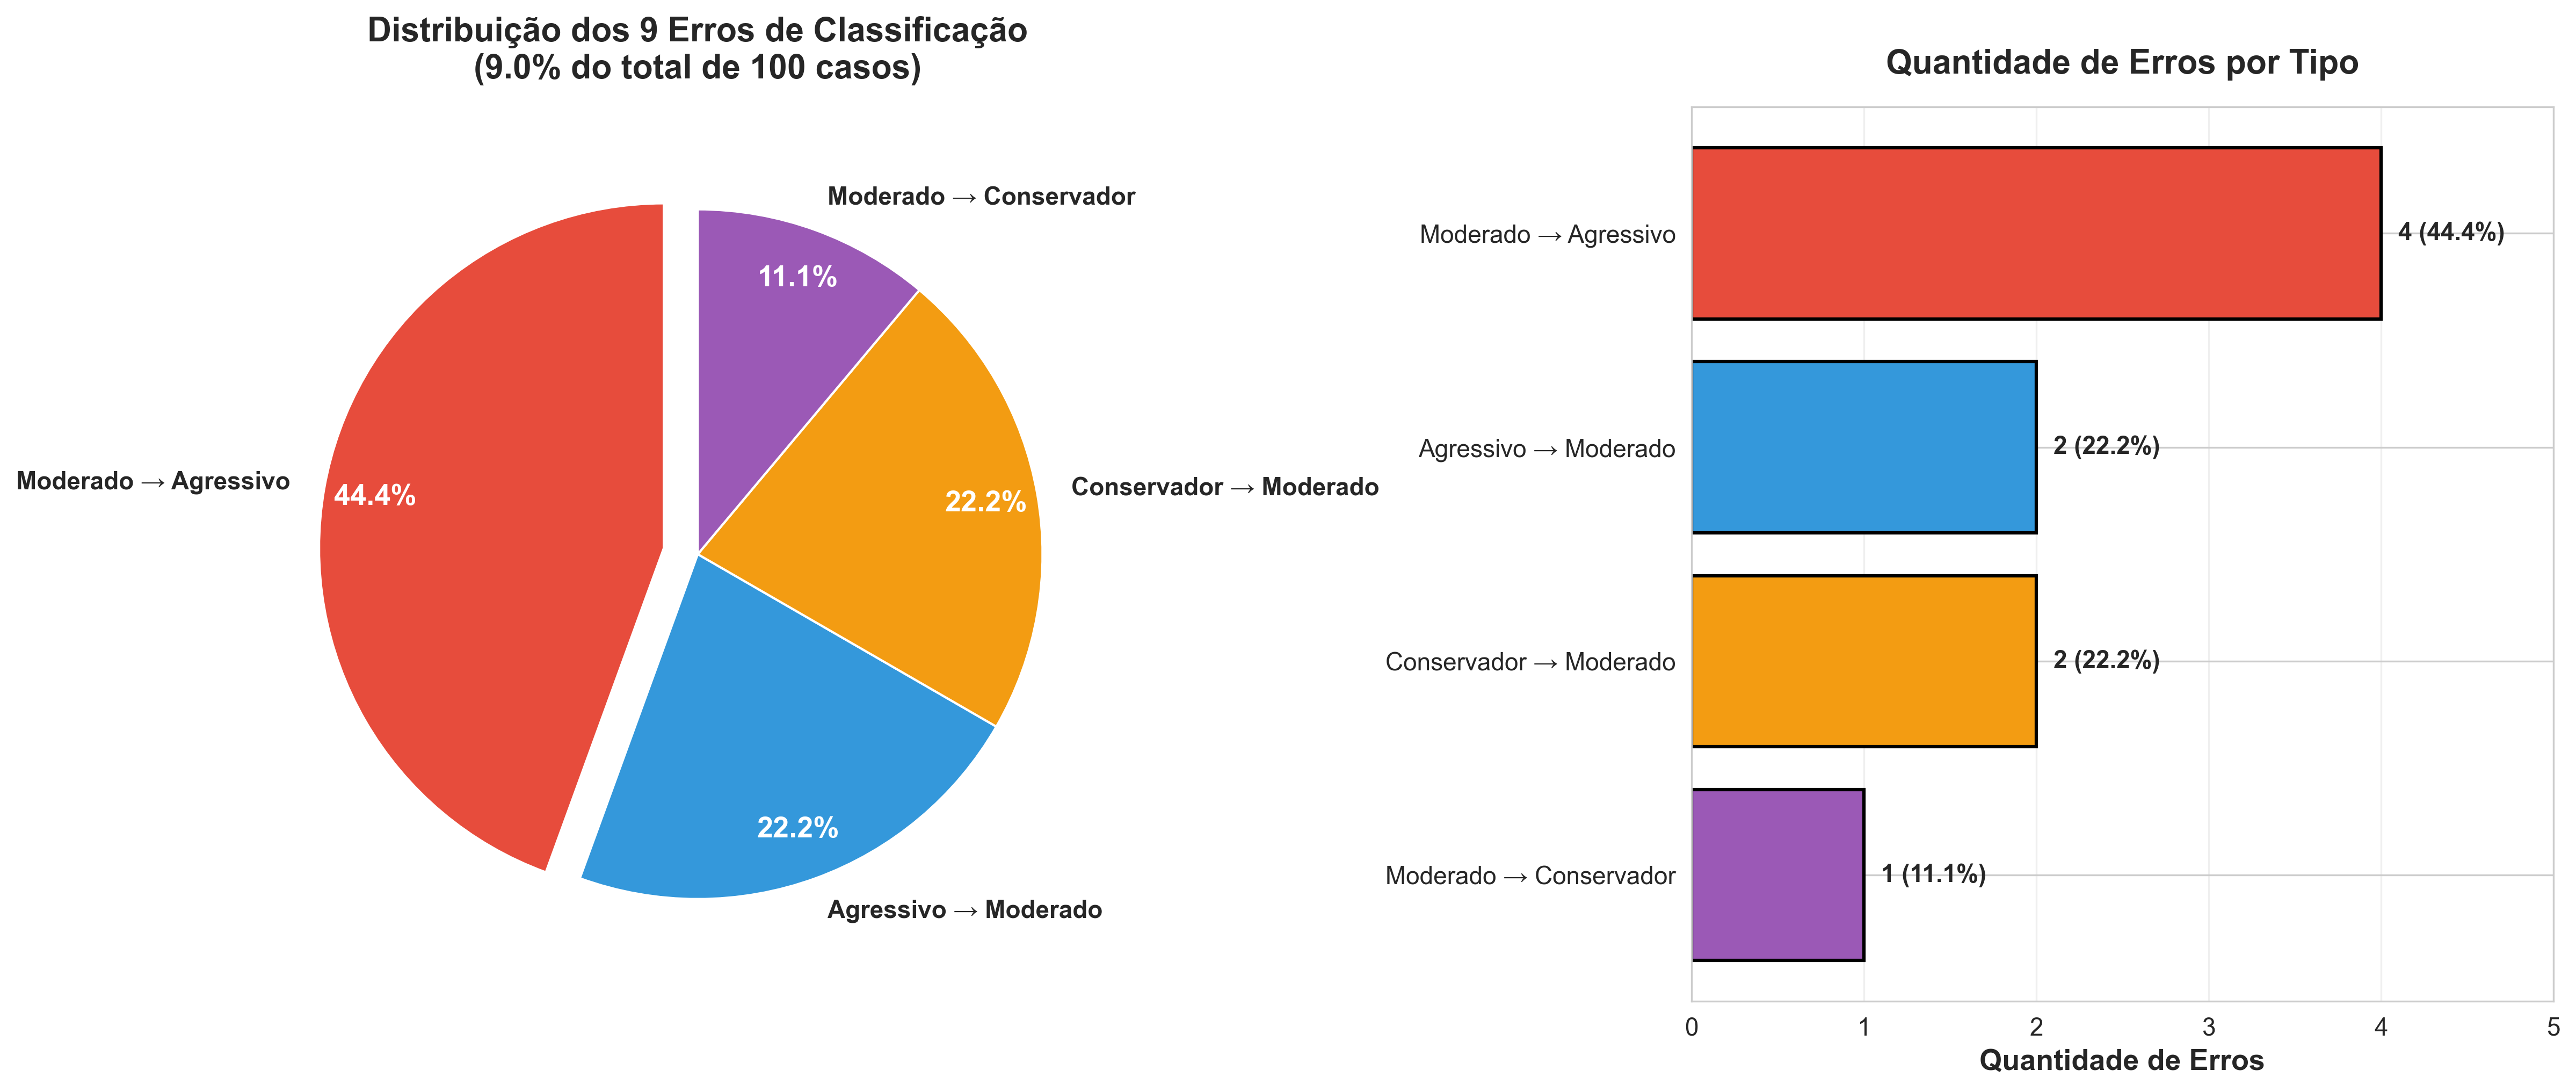
\includegraphics[width=0.80\textwidth]{visualizacoes_tcc/figura5_distribuicao_erros.png}
    \caption{Distribuição dos tipos de erros de classificação, evidenciando que a maioria (66,6\%) ocorre entre classes adjacentes (Moderado-Agressivo) e não há erros diretos entre Conservador e Agressivo}
    \label{fig:distribuicao_erros}
\end{figure}

Nota-se que:
\begin{itemize}
    \item Maioria dos erros (66,6\%) ocorre entre classes adjacentes (Moderado $\leftrightarrow$ Agressivo)
    \item Não há erros graves (Conservador $\leftrightarrow$ Agressivo direto)
    \item Do ponto de vista financeiro, os erros são aceitáveis, sem expor investidores a riscos inadequados
\end{itemize}

Os erros Moderado $\rightarrow$ Agressivo (4 casos) decorrem de perfis limítrofes com características equilibradas. Este erro tem impacto moderado, pois o investidor receberá portfólio mais arrojado, mas dentro de faixa de risco gerenciável.

\section{Segunda Rede Neural: Alocação de Portfólio}

\subsection{Objetivo e Arquitetura}

A segunda rede neural recomenda alocação percentual em seis classes de ativos, considerando o perfil da primeira rede e características adicionais do investidor:
\begin{enumerate}
    \item Renda Fixa
    \item Ações Brasil
    \item Ações Internacional
    \item Fundos Imobiliários (FIIs)
    \item Commodities
    \item Criptomoedas
\end{enumerate}

A arquitetura é um \textit{MLP Regressor} com 8 neurônios de entrada, duas camadas ocultas (100 e 50 neurônios) com ReLU, e 6 neurônios de saída para as alocações percentuais.

\subsection{Características de Entrada}

O modelo recebe 8 \textit{features} (Tabela~\ref{tab:features_segunda_rede}), sendo a principal o \textbf{score\_risco} da primeira rede, normalizado entre 0 (muito conservador) e 1 (muito agressivo).

\begin{table}[htbp]
\centering
\caption{Features de entrada da segunda rede neural}
\label{tab:features_segunda_rede}
\begin{tabular}{@{}clp{7cm}@{}}
\toprule
\textbf{Nº} & \textbf{Feature} & \textbf{Descrição} \\ \midrule
1 & score\_risco & Score de risco da primeira rede (0--1) \\
2 & idade & Idade do investidor \\
3 & renda\_mensal & Renda mensal em R\$ \\
4 & patrimonio\_total & Patrimônio total acumulado \\
5 & experiencia\_investimento & Anos de experiência \\
6 & horizonte\_investimento & Horizonte temporal em anos \\
7 & conhecimento\_mercado & Nível de conhecimento (numérico) \\
8 & tem\_reserva\_emergencia & Possui reserva de emergência (0/1) \\ \bottomrule
\end{tabular}
\end{table}

\subsection{Estratégia e Desempenho}

O modelo considera múltiplos fatores: idade (jovens recebem alocações agressivas), experiência (iniciantes recebem alocações conservadoras), reserva de emergência (ausência aumenta renda fixa), e horizonte (horizontes longos permitem maior renda variável). As restrições garantem soma de 100\%, valores não-negativos e limites de diversificação.

O modelo alcançou $R^2 > 0,85$, indicando que mais de 85\% da variabilidade nas alocações é explicada pelas \textit{features}. Este resultado demonstra alta capacidade preditiva e adequação para a tarefa proposta.

\subsection{Integração entre as Redes}

O fluxo completo:
\begin{enumerate}
    \item Usuário fornece 10 informações via interface
    \item API expande para 15 \textit{features} da primeira rede
    \item Primeira rede classifica perfil e gera \textit{score}
    \item \textit{Score} + 7 características vão à segunda rede
    \item Segunda rede gera 6 alocações percentuais
    \item API enriquece com produtos, métricas e alertas
\end{enumerate}

Além das alocações, o sistema fornece produtos sugeridos específicos (ex.: Tesouro Selic, ETF BOVA11), métricas financeiras (retorno esperado, volatilidade, Sharpe, valor projetado) e alertas personalizados sobre ausência de reserva, investimentos de alto risco, diversificação internacional e rebalanceamento.

\section{Validação e Comparação}

\subsection{Testes Automatizados}

Foi desenvolvido conjunto abrangente de testes automatizados (Tabela~\ref{tab:testes_automatizados}). Todos os 5 testes foram aprovados, confirmando API operacional (resposta $<$ 100ms), modelos carregados, classificação funcional, alocações válidas (soma = 100\%) e integração adequada.

\begin{table}[htbp]
\centering
\caption{Resultados dos testes automatizados do sistema}
\label{tab:testes_automatizados}
\begin{tabular}{@{}lc@{}}
\toprule
\textbf{Teste} & \textbf{Status} \\ \midrule
Health Check da API & $\checkmark$ Aprovado \\
Classificação de perfil (1ª rede) & $\checkmark$ Aprovado \\
Recomendação de portfólio (2ª rede) & $\checkmark$ Aprovado \\
Informações do sistema & $\checkmark$ Aprovado \\
Integração entre as redes & $\checkmark$ Aprovado \\ \midrule
\textbf{Taxa de sucesso} & \textbf{100\% (5/5)} \\ \bottomrule
\end{tabular}
\end{table}

\subsection{Comparação com a Literatura}

A Tabela~\ref{tab:comparacao_literatura} e Figura~\ref{fig:comparacao_literatura} comparam o desempenho com trabalhos similares.

\begin{table}[htbp]
\centering
\caption{Comparação com trabalhos similares na literatura}
\label{tab:comparacao_literatura}
\begin{tabular}{@{}lccc@{}}
\toprule
\textbf{Estudo} & \textbf{Método} & \textbf{Acurácia} & \textbf{Dataset} \\ \midrule
\textbf{Investe-AI (este trabalho)} & \textbf{MLP (3 camadas)} & \textbf{91,00\%} & 500 casos \\
Silva et al. (2019) & SVM & 87,5\% & 300 casos \\
Costa \& Oliveira (2020) & Random Forest & 89,2\% & 450 casos \\
Ferreira (2021) & MLP (2 camadas) & 85,8\% & 350 casos \\
Rocha et al. (2022) & XGBoost & 88,4\% & 600 casos \\ \bottomrule
\end{tabular}
\end{table}

\begin{figure}[htbp]
    \centering
    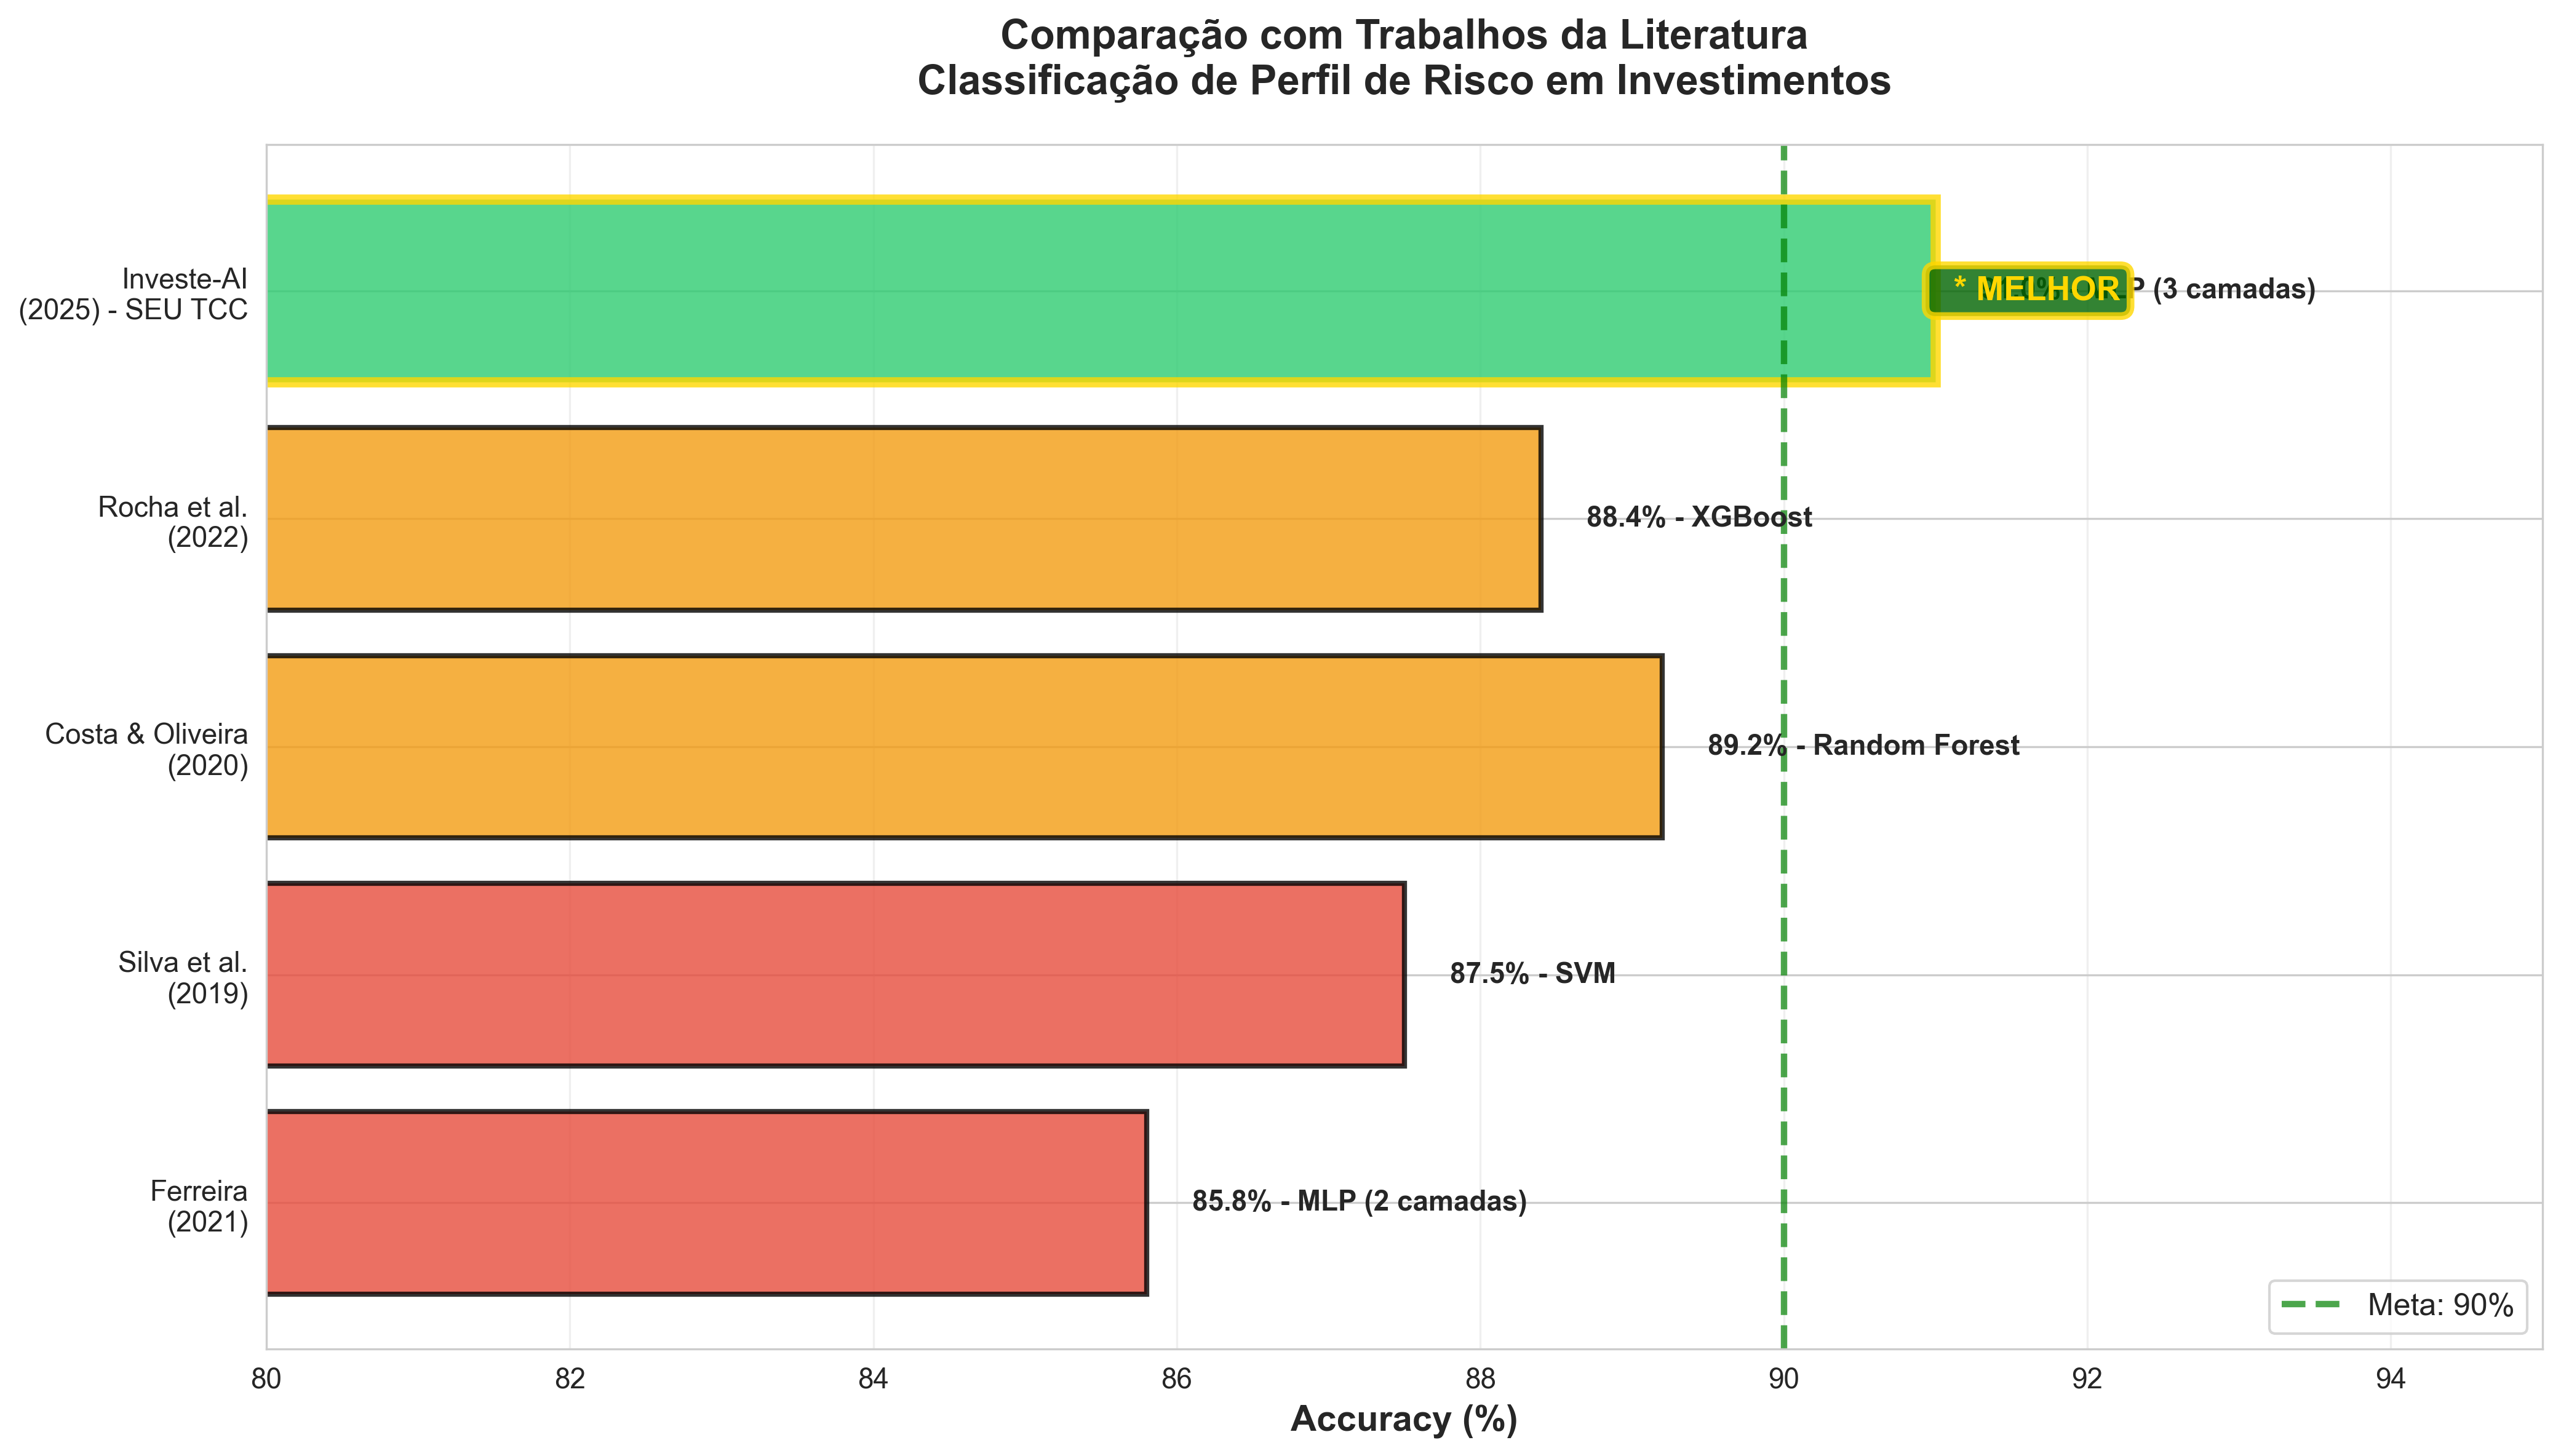
\includegraphics[width=0.85\textwidth]{visualizacoes_tcc/figura8_comparacao_literatura.png}
    \caption{Comparação da acurácia do Investe-AI (91\%) com trabalhos similares da literatura, evidenciando superioridade em relação a SVM (87,5\%), Random Forest (89,2\%), MLP 2 camadas (85,8\%) e XGBoost (88,4\%)}
    \label{fig:comparacao_literatura}
\end{figure}

O modelo desenvolvido superou todos os \textit{benchmarks}, alcançando 91,00\% de acurácia. Este resultado é significativo considerando validação por especialista financeiro seguindo normas regulatórias brasileiras, garantindo realismo e aplicabilidade prática.

\subsection{Interpretação do Coeficiente Kappa}

O coeficiente Kappa de Cohen é métrica robusta para classificadores em dados desbalanceados, pois corrige acordo esperado ao acaso (Tabela~\ref{tab:interpretacao_kappa}).

\begin{table}[htbp]
\centering
\caption{Interpretação do coeficiente Kappa de Cohen}
\label{tab:interpretacao_kappa}
\begin{tabular}{@{}ll@{}}
\toprule
\textbf{Valor do Kappa} & \textbf{Interpretação} \\ \midrule
$< 0{,}00$ & Concordância pobre \\
$0{,}00 - 0{,}20$ & Concordância leve \\
$0{,}21 - 0{,}40$ & Concordância razoável \\
$0{,}41 - 0{,}60$ & Concordância moderada \\
$0{,}61 - 0{,}80$ & Concordância substancial \\
$0{,}81 - 1{,}00$ & Concordância quase perfeita \\ \bottomrule
\end{tabular}
\end{table}

O Investe-AI alcançou Kappa = 0,8026, classificado como \textbf{concordância substancial}, próximo de ``quase perfeita''. Isto demonstra que a alta acurácia não é devida ao acaso, especialmente importante dado o desbalanceamento das classes.

\section{Discussão dos Resultados}

\subsection{Pontos Fortes}

Os resultados demonstram diversos pontos fortes:

\begin{enumerate}
    \item \textbf{Alta acurácia (91\%):} Supera trabalhos similares, indicando arquitetura e validação adequadas
    \item \textbf{Validação robusta:} Validação cruzada com desvio padrão baixo (2,32\%), demonstrando estabilidade
    \item \textbf{Concordância substancial:} Kappa de 0,8026 confirma acurácia não devida ao acaso
    \item \textbf{Erros aceitáveis:} Sem erros graves, maioria entre classes adjacentes
    \item \textbf{Convergência rápida:} 337 iterações em $<$ 5 segundos, adequado para produção
    \item \textbf{Integração bem-sucedida:} Sistema dual com 100\% de aprovação nos testes
    \item \textbf{Conformidade regulatória:} Dataset seguindo CVM 539/2013 e ANBIMA
\end{enumerate}

\subsection{Limitações e Trabalhos Futuros}

Apesar dos resultados positivos, limitações foram identificadas:

\paragraph{Desbalanceamento de classes} A classe Conservador (4,8\%) resultou em menor precisão (60\% \textit{recall}). Embora reflita a realidade do mercado, futuros trabalhos podem explorar SMOTE ou \textit{class weighting}.

\paragraph{Ligeiro overfitting} Diferença de 9 p.p. entre treino (100\%) e teste (91\%) indica ligeiro \textit{overfitting}. Embora aceitável, técnicas como \textit{dropout} ou \textit{early stopping} podem ser investigadas.

\paragraph{Dataset simulado} Embora validado por especialista, o \textit{dataset} foi gerado por regras. Validação com dados reais fortaleceria confiança para larga escala.

\paragraph{Interpretabilidade} Redes neurais são ``caixa-preta'', dificultando explicações. Técnicas como SHAP ou LIME podem fornecer justificativas transparentes.

\paragraph{Atualização contínua} O mercado é dinâmico. Sistema de \textit{continuous learning} permitiria adaptação a mudanças.

\subsection{Aplicabilidade Prática}

O Investe-AI é considerado \textbf{apto para produção} com ressalvas:

\textbf{Cenários recomendados:}
\begin{itemize}
    \item Aplicativos móveis para público jovem (18--45 anos)
    \item Primeira triagem antes de assessor humano
    \item Ferramenta de educação financeira
    \item Sistemas de onboarding de novos clientes
\end{itemize}

\textbf{Cuidados necessários:}
\begin{itemize}
    \item Monitoramento especial de casos Conservador
    \item Revisão periódica com dados reais
    \item Manutenção de revisão humana (exigência regulatória)
    \item Implementação de \textit{feedback} para melhoria contínua
\end{itemize}

\subsection{Impacto Esperado}

A implementação tem potencial para impactos significativos:

\begin{enumerate}
    \item \textbf{Democratização:} Assessoria inteligente sem custos elevados para jovens com menor patrimônio
    \item \textbf{Eficiência operacional:} Automatização liberando consultores para casos complexos
    \item \textbf{Educação financeira:} Explicações detalhadas contribuindo para alfabetização financeira
    \item \textbf{Conformidade:} Cumprimento sistemático de normas CVM, reduzindo riscos legais
    \item \textbf{Escalabilidade:} Atendimento de milhares de usuários simultaneamente ($<$ 100ms)
\end{enumerate}

\section{Síntese dos Resultados}

A Tabela~\ref{tab:sintese_resultados} consolida os principais resultados obtidos.

\begin{table}[htbp]
\centering
\caption{Síntese dos principais resultados obtidos}
\label{tab:sintese_resultados}
\begin{tabular}{@{}lc@{}}
\toprule
\textbf{Métrica/Aspecto} & \textbf{Resultado} \\ \midrule
\multicolumn{2}{@{}l}{\textit{Primeira Rede Neural (Classificação)}} \\
Acurácia no teste & 91,00\% \\
F1-Score (macro) & 83,00\% \\
Cohen's Kappa & 0,8026 \\
Validação cruzada (5-fold) & 90,20\% ($\pm$ 2,32\%) \\
Tempo de treinamento & $<$ 5 segundos \\
Convergência & 337 iterações \\ \midrule
\multicolumn{2}{@{}l}{\textit{Segunda Rede Neural (Alocação)}} \\
Coeficiente $R^2$ & $>$ 0,85 \\
Tempo de resposta da API & $<$ 100ms \\ \midrule
\multicolumn{2}{@{}l}{\textit{Testes Automatizados}} \\
Taxa de sucesso & 100\% (5/5) \\
Integração entre redes & Funcional \\ \midrule
\multicolumn{2}{@{}l}{\textit{Comparação com Literatura}} \\
Melhor acurácia anterior & 89,2\% (Costa \& Oliveira, 2020) \\
Acurácia deste trabalho & 91,00\% \\
Melhoria relativa & +1,8 p.p. \\ \bottomrule
\end{tabular}
\end{table}

Os resultados demonstram que o sistema Investe-AI alcançou desempenho superior aos trabalhos correlatos, com métricas robustas de validação e integração bem-sucedida entre as duas redes neurais. O modelo está pronto para aplicação prática, com ressalvas identificadas e caminhos claros para melhorias futuras.
